%% ----------------------------------------------------------------
%% Thesis.tex -- MAIN FILE (the one that you compile with LaTeX)
%% ----------------------------------------------------------------
% Set up the document
\documentclass[11pt,a4paper,english,greek,twoside]{Thesis}
\usepackage{standalone}
%All packages are loaded inside Thesis.cls
%% ----------------------------------------------------------------

\makeatletter
\def\maxwidth#1{\ifdim\Gin@nat@width>#1 #1\else\Gin@nat@width\fi}
\makeatother

% Set up the Title Page
\title{Ανάπτυξη Διεπαφής Εγκεφάλου - Υπολογιστή με την χρήση Steady State Evoked Potentials (SSVEP)}
%\subtitle{υπότιτλος}
\authors{{Χριστόδουλου Θ. Μπενετάτου}}

\date{\the\month/\the\year}
\setcounter{secnumdepth}{3}


\begin{document}
\frontmatter      % Begin Roman style (i, ii, iii, iv...) page numbering
\maketitle
% ----------------------------------------------------------------

\setstretch{1.3}  % It is better to have smaller font and larger line spacing than the other way round

% Define the page headers using the FancyHdr package and set up for one-sided printing
\fancyhead{}  % Clears all page headers and footers
\rhead{\thepage}  % Sets the right side header to show the page number
\lhead{}  % Clears the left side page header

\pagestyle{fancy}  % Finally, use the "fancy" page style to implement the FancyHdr headers

% ----------------------------------------------------------------



%% ----------------------------------------------------------------
% The "Funny Quote Page"
% \pagestyle{empty}  % No headers or footers for the following pages
%
% \null\vfill
% % Now comes the "Funny Quote", written in italics
% \textit{``Write a funny quote here.''}
%
% \begin{flushright}
% If the quote is taken from someone, their name goes here
% \end{flushright}
%
% \vfill\vfill\vfill\vfill\vfill\vfill\null
% \clearpage  % Funny Quote page ended, start a new page
%% ----------------------------------------------------------------

% The Abstract Page
%\chapter{Περίληψη}  % Add the "Abstract" page entry to the Contents
%\addtocontents{toc}{\vspace{1em}}  % Add a gap in the Contents, for aesthetics

% \abstract{
\chapter{Περίληψη}
\par Ο βασικός στόχος-κίνητρο της παρούσας διπλωματικής εργασίας είναι η μελέτη της καταλληλότητας του οικονομικού εγκεφαλογράφου Emotiv Epoc, για την υλοποίηση μιας διεπαφής εγκεφάλου-υπολογιστή (BCI) κάνοντας χρήση των οπτικών προκλητών δυναμικών σταθερής κατάστασης (SSVEP). Πρώτο στάδιο της διεπαφής, είναι η κατασκευή της συσκευής που παρέχει τις απαραίτητες επαναλαμβανόμενες οπτικές διεγέρσεις (ΕΟΔ). Κατασκευάζουμε ένα πάνελ αποτελούμενο από 4 LED συστοιχίες, καθώς και το κύκλωμα οδήγησης τους, το οποίο επιτρέπει την ανεξάρτητη επιλογή συχνότητας και duty cycle, για κάθε συστοιχία. Στο επόμενο στάδιο, δημιουργούμε μια εφαρμογή η οποία υλοποιεί το πρωτόκολλο καταγραφής των δεδομένων που σχεδιάσαμε, ελέγχοντας πλήρως την παραγωγή των οπτικών διεγέρσεων παρέχοντας παράλληλα στον χρήστη οπτικές και ακουστικές οδηγίες για να εξασφαλιστεί η τήρηση του πρωτοκόλλου. Επιπλέον σχεδιάζουμε μια γραφική διεπαφή χρήστη βασιζόμενη σε open source λογισμικό, για την real-time παρακολούθηση του εγκεφαλογραφήματος, καθώς και του συχνοτικού περιεχομένου για κάθε κανάλι. Στα SSVEP δεδομένα που συλλέξαμε, πειραματιζόμαστε με διάφορες μεθόδους εξαγωγής χαρακτηριστικών και ταξινόμησης, που χρησιμοποιούνται στην βιβλιογραφία, καθώς και δικές μας παραλλαγές τους, και επιτυγχάνουμε επιδόσεις έως και 90\% ακρίβεια με ITR 20.58 bits/min, που συμβαδίζουν με τις state of the art επιδόσεις διεπαφών που κάνουν χρήση αντίστοιχου υλικού. Τέλος, υλοποιούμε το online σκέλος της διεπαφής, ένα ασύγχρονο σύστημα πραγματικού χρόνου, στο οποίο οι χρήστες καλούνται να κατευθύνουν, μέσα σε έναν εικονικό λαβύρινθο, το avatar τους, προς έναν επιθυμητό στόχο.
 \\\\\\
 \large{\textbf{Λέξεις-Κλειδιά}}\\
 Διεπαφές Εγκεφάλου - Υπολογιστή, Οπτικά Προκλητά Δυναμικά Σταθερής Κατάστασης, Ανάλυση Κανονικής Συσχέτισης, Self-Paced BCI (ασύγχρονη διεπαφή)
 
 %}
 \clearpage  % Abstract ended, start a new page



%\chapter{Abstract}  % Add the "Abstract" page entry to the Contents
%\addtocontents{toc}{\vspace{1em}}  % Add a gap in the Contents, for aesthetics
 %\abstracteng{
 \chapter{Abstract}
\par
 The main purpose of this diploma thesis, is to study whether an inexpensive non-medical graded EEG headset, like Emotiv Epoc, is suitable for implementing a Brain Computer Interface (BCI), based on Steady State Visual Evoked Potentials (SSVEP). First stage of the implementation, is the creation of the device that provides the necessary repeated visual stimuli (RVS). We build, a panel made of four LED arrays, and its driving circuit, which allows the independent selection of stimulus frequency and duty cycle, for every RVS. The next stage, consists of the creation of a application that implements the offline EEG data recording protocol that we designed, which is able to fully control the RVS, and at the same time, providing all the necessary visual and audio cues to the user, in order to follow the protocol. Additionally, we design a Graphical User Interface based in open-source software, for the real-time monitoring of every channel of the EEG signal, in time and frequency domain. During the offline processing, we experiment wιth various methods of feature extraction and classification, as well as some of our modifications of them, and we achieve perfomance up to 90\% accuracy and 20.58 bits/min ITR, results that comfort to the state of the art perfomances of BCIs that use similar materials. Finally, we implement the online part of the BCI, an asynchronous real-time system, where users are asked to navigate their avatar to a desired target, through a virtual maze.
 \\\\\\
 \large{\textbf{Keywords}}\\
Brain Computer Interfaces (BCIs), Steady State Visual Evoked Potentials (SSVEP), Canonical Correlation Analysis (CCA), Self-Paced BCI (asynchronous).
 %}
 \clearpage  % Abstract ended, start a new page

%% ----------------------------------------------------------------

\setstretch{1.3}  % Reset the line-spacing to 1.3 for body text (if it has changed)

% The Acknowledgements page, for thanking everyone
\acknowledgements{
\addtocontents{toc}{\vspace{1em}}  % Add a gap in the Contents, for aesthetics

}
\clearpage  % End of the Acknowledgements
%% ----------------------------------------------------------------

\pagestyle{fancy}  %The page style headers have been "empty" all this time, now use the "fancy" headers as defined before to bring them back

%% ----------------------------------------------------------------
\lhead{\emph{Περιεχόμενα}}  % Set the left side page header to "Contents"
\tableofcontents  % Write out the Table of Contents


%% ----------------------------------------------------------------
\lhead{\emph{Κατάλογος Εικόνων και Σχημάτων}}  % Set the left side page header to "List if Figures"
\listoffigures  % Write out the List of Figures

%% ----------------------------------------------------------------
\lhead{\emph{Κατάλογος Πινάκων}}  % Set the left side page header to "List of Tables"
\listoftables  % Write out the List of Tables

%% ----------------------------------------------------------------
\mainmatter	  % Begin normal, numeric (1,2,3...) page numbering
\pagestyle{fancy}  % Return the page headers back to the "fancy" style

% Include the chapters of the thesis, as separate files
% Just uncomment the lines as you write the chapters
\lhead{\emph{Κεφάλαιο 1}}

%% !TEX root = ../Thesis.tex
%% !TEX output_directory
\documentclass[11pt,a4paper,english,greek,twoside]{../Thesis}
\begin{document}
\chapter{Εισαγωγή}
\section{Σημασία Μελέτης Εγκεφάλου και Βιοηλεκτρικών Σημάτων}
%βαλε και μια εικονα
\section{Σκοπός και Συνεισφορά της Διπλωματικής Εργασίας}
Στόχος αυτής της διπλωματικής εργασίας είναι η υλοποίηση μιας διεπαφής εγκεφάλου υπολογιστή βασιζόμενη σε μια κατηγορία οπτικών προκλητών δυναμικών που ονομάζονται Steady State Visual Evoked Potentials. Σε αντίθεση όμως με την πλειοψηφία της έρευνας σε αυτόν τον τομέα, όπου γίνεται χρήση ακριβών εγκεφαλογράφων κατασκευασμένων για ιατρική χρήση, σε αυτή την εργασία γίνεται χρήση ενός low-budget εγκεφαλογράφου, πράγμα που αποτελεί και την βασική πρόκληση της εργασίας. Η όλη πειραματική διαδικασία, το hardware για την δημιουργία των οπτικών ερεθισμάτων, η γραφική διεπαφή για την παρακολούθηση των εγκεφαλικών σημάτων σε πραγματικό χρόνο, καθώς και ένα σύνολο συναρτήσεων για την επεξεργασία των εγκεφαλικών σημάτων στην προγραμματιστική γλώσσα Python, σχεδιάστηκαν και υλοποιήθηκαν εξολοκλήρου στα πλαίσια της εργασίας. Επιπλέον, δημιουργήσαμε ένα dataset με όλες τις καταγραφές εγκεφαλογραφήματος που έλαβαν μέρος κατά την διάρκεια της εργασίας, ταξινομημένες ανά άτομο, έτσι ώστε όλα αυτά μαζί να αποτελέσουν εφαλτήριο για περαιτέρω έρευνα πάνω στο συγκεκριμένο θέμα. Όσον αφορά τους αλγορίθμους που χρησιμοποιήθηκαν για την εξαγωγή πληροφορίας από τα εγκεφαλικά σήματα, δοκιμάστηκαν διάφορες μέθοδοι που χρησιμοποιούνται κατά κόρον στην βιβλιογραφία, και είδαμε πως στην offline επεξεργασία των σημάτων, η απόδοση του συστήματος συγκρίνεται με τις state-of-the-art επιδόσεις για low-budget εγκεφαλογράφους, έχοντας όμως πολλά περιθώρια μέχρι να συγκριθεί με τις επιδόσεις πιο ακριβών. Τέλος \textcolor{red}{ΠΕΣ ΤΙ ΘΑ ΚΑΝΕΙΣ ΜΕ ΤΟ REAL TIME}

\section{Διάρθρωση Διπλωματικής Εργασίας}
\par Η εργασία ακολουθεί την εξής πορεία:
\begin{itemize}
	\item Στο κεφάλαιο 2 παρουσιάζεται η σχεδίαση του συνολικού συστήματος και των υπομονάδων του, καθώς και το σύνολο δεδομένων στο οποίο εργαζόμαστε. Γίνεται συσχέτιση με άλλες μεθόδους οι οποίες έχουν σχέση με την εργασία μας, ενώ αφήνουμε τις λεπτομέρειες κάθε υποσυστήματος για να παρουσιαστούν ξεχωριστά.
	\item Στο κεφάλαιο 3 παρουσιάζεται το ζήτημα της αναγνώρισης δράσεων με αξιοποίηση μόνο οπτικής πληροφορίας και εξηγείται η λειτουργία του υποσυστήματος Όρασης Χαμηλού Επιπέδου. Αναλύεται η μέθοδος των Πυκνών Τροχιών \cite{wang_2011} και μια επέκτασή της που λαμβάνει υπόψιν της επιπλέον χαρακτηριστικά πόζας \cite{rohrbach_2012}. Τέλος, περιγράφουμε τη σύνδεση αυτών των εργασιών στη δική μας σχεδιαστική επιλογή.
	\item Στο κεφάλαιο 4 παρουσιάζεται το ζήτημα της ανίχνευσης αντικειμένων και η σύνδεσή του με το σημασιολογικό υποσύστημα. Στη σημασιολογία εντάσσουμε και το υποσύστημα ακουστικής πληροφορίας, οπότε δεν αφιερώνουμε για αυτό ξεχωριστό κεφάλαιο. Γίνεται μια ιστορική επισκόπηση της ανίχνευσης αντικειμένων και προσκηνίου, παρουσιάζεται η μέθοδος των Μοντέλων Παραμορφώσιμων Τμημάτων \cite{felzenszwalb_2008}, των Μοντέλων Μίξης Γκαουσιανών για εξαγωγή προσκηνίου και η Μέθοδος Ταιριάσματος στην ανίχνευση αντικειμένου οπτικά και γλωσσικά. Δικαιολογούμε τις σχεδιαστικές μας επιλογές και παρουσιάζουμε αποτελέσματα ανίχνευσης συνδυάζοντας γλωσσική και οπτική πληροφορία.
	\item Στο κεφάλαιο 5 παρουσιάζεται η διαδικασία εξαγωγής πληροφορίας για τον τύπο λαβής (grasping type) στα frames του βίντεο ως επιπλέον αναγνωριστικό χαρακτηριστικό. Παρουσιάζονται θέματα από την περιοχή των Συνελικτικών Νευρωνικών Δικτύων και η από αρχής υλοποίηση ενός συστήματος ανίχνευσης χεριών.
	\item Στο κεφάλαιο 6 γίνεται ανάλυση των αλγορίθμων και των αποτελεσμάτων ταξινόμησης. Εδώ συγκρίνουμε όλες τις μεθόδους και τα αποτελέσματά μας με άλλες εργασίες.
	\item Στο κεφάλαιο 7 αναπτύσσουμε μια νέα μέθοδο κατάτμησης δράσεων και δείχνουμε τα πειραματικά αποτελέσματα για αυτή πάνω σε βίντεο του συνόλου δεδομένων μας.
	\item Στο κεφάλαιο 8, κλείνουμε αυτή την εργασία παρουσιάζοντας τις συνεισφορές μας και προτείνοντας μελλοντικές ερευνητικές κατευθύνσεις.
\end{itemize}

\end{document}
 % Introductionaa

\lhead{\emph{Κεφάλαιο 2}}

    % !TEX root = ../Thesis.tex
% !TEX output_directory
\documentclass[11pt,a4paper,english,greek,twoside]{../Thesis}
%\usepackage{subfig}
%\usepackage{subcaption} 
%\usepackage[demo]{graphicx}
%\usepackage{caption}
% \renewcommand\paragraph{\@startsection{paragraph}{4}{\z@}%
%                                     {-3.25ex \@plus1ex \@minus.2ex}% original: without the minus
%                                     {1.5ex plus .2ex}% original {-1em}%
%                                     {\normalfont\normalsize\bfseries}}
\begin{document}
\chapter{Ηλεκτροεγκεφαλογραφία}
\section{Βιοηλεκτρικά Σήματα και Ηλεκτροεγκεφαλογράφημα}
\par Τα βιοηλεκτρικά σήματα είναι το αποτέλεσμα των ηλεκτροχημικών μεταβολών που λαμβάνουν χώρα εντός και μεταξύ των κυττάρων των νεύρων καθώς και των μυών. Πιο συγκεκριμένα, εάν ένα τέτοιο κύτταρο δεχθεί ερέθισμα ισχυρότερο από ένα κατώφλι συνήθως μεταξύ  -55mV και -50mV, τότε θα παράγει ένα δυναμικό δράσης το οποίο θα μεταδοθεί και θα διεγείρει γειτονικά κύτταρα. Αυτή η ομαδική δραστηριότητα των κυττάρων παράγει ηλεκτρικά πεδία ικανά να ανιχνευτούν με την βοήθεια ηλεκτροδίων τα οποία τοποθετούνται στην επιφάνεια του αντίστοιχου οργάνου, είτε στην δερματική επιφάνεια πάνω αυτό το όργανο. Όταν το ζωτικό αυτό όργανο είναι ο εγκέφαλος τότε το βιοηλεκτρικό σήμα ονομάζεται Ηλεκτροεγκεφαλογράφημα (ΗΕΓ – EEG) και η πρώτη καταγραφή ΗΕΓ, έγινε το 1924 από τον Γερμανό ψυχίατρο Hans Berger \cite{berger1924innervation}. 

\par Η Ηλεκτροεγκεφαλογραφία, είναι η πρώτη μέθοδος που χρησιμοποιήθηκε για την απεικόνιση της εγκεφαλικής δραστηριότητας, πριν την εμφάνιση μεθόδων όπως η μαγνητική τομογραφία (MRI) και τομογραφία εκπομπής ποζιτρονίων (PET). Παρουσιάζει σημαντικά πλεονεκτήματα όπως το ότι είναι πολύ οικονομικά προσιτή μέθοδος, συγκρινόμενη με τις άλλες που αναφέρθηκαν, και το γεγονός πως έχει πολύ χρονική ανάλυση (temporal resolution), καθώς ο χρόνος μεταξύ της παραγωγής του νευρικού σήματος, και της προκαλούμενης μεταβολής δυναμικού είναι πρακτικά αμελητέος. Ωστόσο, όσον αφορά την χωρική ανάλυση (spatial resolution), δεν ισχύει κάτι αντίστοιχο. Τα ηλεκτρικά σήματα από την στιγμή που ξεκινάνε από την πηγή τους, μέχρι να καταλήξουν στα ηλεκτρόδια, διασκορπίζονται κατά την διέλευση τους από το κρανίο. Συνεπώς το σήμα που ανιχνεύεται από ένα ηλεκτρόδιο σε μια συγκεκριμένη περιοχή δεν προέρχεται μόνο από το σημείο του εγκεφάλου που καλύπτει, αλλά και από τα γειτονικά. Αυτό το πρόβλημα μπορεί να αντιμετωπιστεί κάνοντας χρήση περισσότερων ηλεκτροδίων, και χρήσης τεχνικών χωρικού φιλτραρίσματος, για την λύση του αντίστροφου προβλήματος, δηλαδή την εύρεση του πραγματικού ηλεκτρικού σήματος που ξεκίνησε από κάθε περιοχή του εγκεφάλου. Ένας άλλος τρόπος είναι να χρησιμοποιηθούν ηλεκτρόδια που εισχωρούν σε μεγαλύτερο βάθος, πλησιάζοντας την πηγή του σήματος, πριν αυτό αλλοιωθεί από το κρανίο, προσφέροντας πολύ καλύτερη χωρική ανάλυση. Το εγκεφαλογράφημα που κάνει χρήση τέτοιου τύπου ηλεκτρόδια, ονομάζεται επεμβάτικο (invasive EEG).
\section{Εγκεφαλογράφος}
\par Η συσκευή που χρησιμοποιείται για την καταγραφή του εγκεφαλογραφήματος, ονομάζεται εγκεφαλογράφος, και είναι μια πολύπλοκη συσκευή με διάφορα υποσυστήματα. Από τις αρχές του 20ου αιώνα που δημιουργήθηκε ο πρώτος εγκεφαλογράφος, μέχρι σήμερα, έχουν υπάρξει δραματικές αλλαγές στον τρόπο υλοποίησης τους, με ποιο σημαντική την εισαγωγή της ψηφιακής τεχνολογίας στην αλυσίδα επεξεργασίας του σήματος. Τα υποσυστήματα που παραθέτονται στην συνέχεια, περιέχονται σε όλους τους σύγχρονους εγκεφαλογράφους, χωρίς να σημαίνει πως δεν υπάρχουν παραλλαγές και επιπλέον υποσυστήματα σε άλλους.
\begin{figure}
\centering     %%% not \center
 \subfigure[]{\label{subfig:a}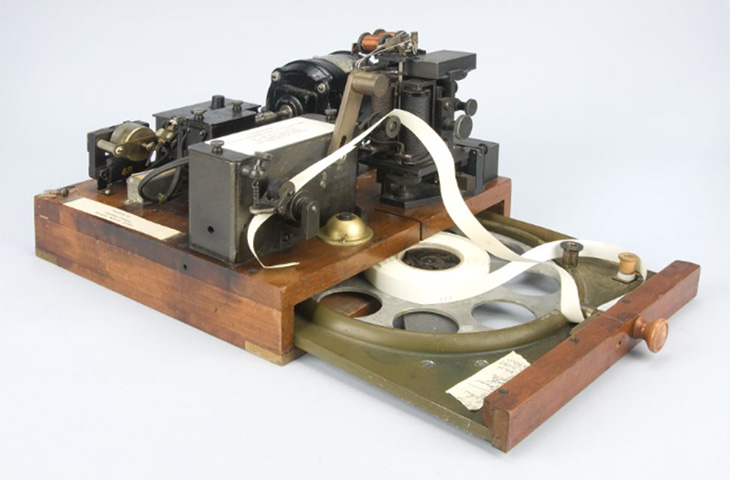
\includegraphics[width=80mm]{{{ImagesSSVEP/firstEEG}.jpg}}}
\subfigure[]{\label{subfig:b}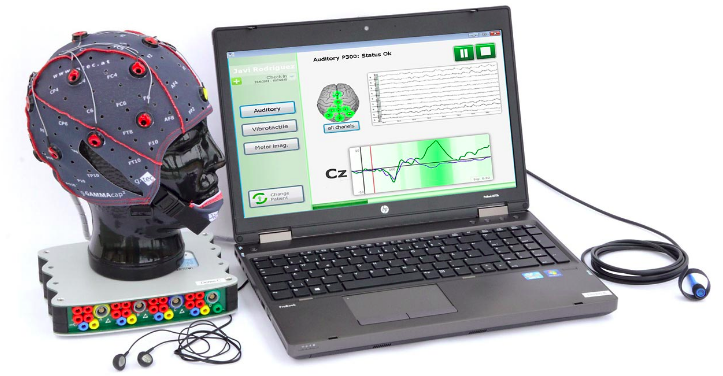
\includegraphics[width=80mm]{{{ImagesSSVEP/gtec_EEG_2}.png}}}
\caption{Εικόνα (α), Η πρώτη συσκευή καταγραφής ΗΕΓ που κατέγραφε την κυματομορφή σε ταινία χαρτιού \cite{garceau1934amplifier, Gfa_undated-vb}. Εικόνα (β), O υπερσύγχρονος εγκεφαλογράφος της g.tec, μπορεί να καταγράφει ταυτόχρονα δεδομένα από 128 ηλεκτρόδια, ο ενισχυτής αναλαμβάνει την ενίσχυση και ψηφιοποίηση των σημάτων, τα οποία στέλνονται στην μονάδα επεξεργασίας και απεικόνισης. }
\end{figure}
\subsection{Ηλεκτρόδια}
  \par Tα ηλεκτρόδια στην πραγματικότητα, είναι μετατροπείς, οι οποίοι ανιχνεύουν την κατανομή των ιόντων στην επιφάνεια των ιστών που καλύπτουν, μετατρέποντας το ιοντικό ρεύμα σε ρεύμα ηλεκτρόνιων. Τα ηλεκτρόδια χωρίζονται σε δύο βασικές κατηγορίες, τα 'υγρά' (wet) και τα 'στεγνά' (dry) και καθένα από αυτά μπορεί να είναι είτε μιας χρήσης, είτε επαναχρησιμοποιούμενο. Ένα ακόμα κριτήριο που τα διαφοροποιεί είναι ενεργά η παθητικά, αν δηλαδή κατασκευάζονται με έναν ενισχυτή ενσωματωμένο στο ίδιο πακέτο (ενεργά), η όχι (παθητικά).
\begin{itemize}
    \item{Υγρά (Wet) Ηλεκτρόδια}
    \par Αυτού του τύπου τα ηλεκτρόδια είναι κατά κύριο λόγω παθητικά, και χρησιμοποιείται αγώγιμο υγρό μεταξύ του δέρματος και του ηλεκτροδίου προκειμένου να επιτευχθεί αποδεκτή αντίσταση επαφής, η οποία κυμαίνεται μεταξύ $5kΩ$ και $20kΩ$ \cite{Nunez2006-li}, έτσι ώστε να εξασφαλιστεί καλή ποιότητα σήματος ΗΕΓ με υψηλό λόγο σήματος προς θόρυβο (SNR). Ο συχνότερος τύπος 'υγρών' ηλεκτροδίων είναι τα αργύρου-χλωριούχου αργύρου (Ag – AgCL) \ref{fig:wet_elec}, τα οποία αποτελούνται από ένα δισκίο, από καθαρό άργυρο $99.9\% $, επικαλυμμένα από ένα λεπτό στρώμα χλωριούχου αργύρου. Είναι ευρέως χρησιμοποιούμενα λόγω του χαμηλού κόστους τους, της ευκολίας στην χρήση τους, καθώς και το ότι δεν είναι τοξικά.  
    \par Ένα άλλο είδος υγρών ηλεκτροδίων, χρησιμοποιούνται στον εγκεφαλογράφο Epoc που κατασκευάζεται από την εταιρεία Emotiv, και αποτελούνται από ένα χάλκινο ηλεκτρόδιο, επικαλυμμένο από μια λεπτή στρώση χρυσού. Η επαφή με το δέρμα γίνεται μέσω ενός κυλινδρικού σφουγγαριού (felt pad), το οποίο διαποτίζετε σε αλατούχο διάλυμα (saline) για την ελάττωση της αντίστασης επαφής.
    \par Παρότι η επίδοση των υγρών ηλεκτροδίων είναι πολύ ικανοποιητική, και χρησιμοποιείται ως σημείο αναφοράς για τις νέες τεχνολογίες ηλεκτροδίων που εμφανίζονται, μια σειρά από μειονεκτήματα, εμποδίζει την χρήση τους σε περιβάλλοντα εκτός εργαστηρίου. Το πρώτο και βασικότερο είναι η δυσκολία που έχουν στην εφαρμογή τους και η άβολη αίσθηση που έχουν κατά την χρήση τους λόγω του υγρού στοιχείου. Συνήθως, απαιτείται ειδικός καθαρισμός  του σημείου επαφής πριν την χρήση, για την επίτευξη καλύτερου σήματος, αλλά και μετά το πέρας της διαδικασίας, για να καθαριστεί το δέρμα από  τα υπολείμματα του αγώγιμου υγρού. Επιπλέον, η επίτευξη της επιθυμητής αντίστασης που αναφέρθηκε προηγουμένως, μπορεί να καθυστερήσει σημαντικά. Τέλος, λόγω της πτητικότητας του αγώγιμου υγρού, υπάρχει ένα μικρό περιθώριο λίγων ωρών, πριν να ξαναχρειαστεί να το ανανεώσουμε.
    
    \begin{figure}[h]
    \centering
    \noindent\makebox[\textwidth]{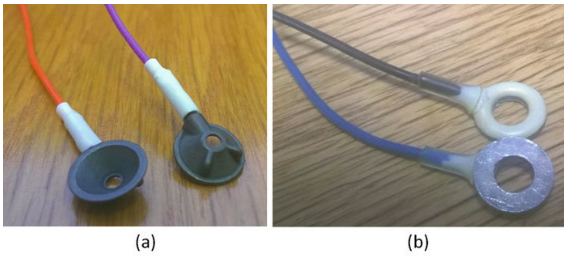
\includegraphics[scale=0.6]{{ImagesSSVEP/wet_elec}.png}}
    \captionsetup{singlelinecheck = false, justification=justified} % used for left alignment
    \caption{Δύο ηλεκτρόδια αργύρου-χλωριούχου αργύρου (Ag – AgCL), ένα μίας χρήσης (a) και ένα επαναχρησιμοποιούμενο (b). Εικόνα από \cite{Casson2018-fn}}
    \label{fig:wet_elec}
    \end{figure}
    \item{Στεγνά (Dry) Ηλεκτρόδια}
    \par Τα προηγούμενα μειονεκτήματα έρχεται να τα καλύψει μια νέα τεχνολογία ηλεκτροδίων που δεν χρησιμοποιούν κάποιο αγώγιμο υγρό, αλλά εκμεταλλευόμενα τις εξελίξεις στον τομέα τεχνολογίας υλικών και των μικρο-συστημάτων (MEMS), προσπαθούν να επιτύχουν ποιότητα σήματος συγκρίσιμη με αυτή των υγρών ηλεκτροδίων. Λόγω της έλλειψής αγώγιμου υγρού, η αντίσταση επαφής μεταξύ των ηλεκτροδίων και του δέρματος είναι πολύ μεγαλύτερη σε σχέση με τα υγρά ηλεκτρόδια, συνεπώς κατά κύριο λόγο είναι ενεργά, καθώς περιέχουν και έναν χαμηλής ενέργειας ενισχυτή οργανολογίας (instrumental amplifier) με πολύ υψηλή αντίσταση εισόδου, προκειμένου να υπάρχει όσο το δυνατόν μικρότερη απώλεια σήματος. Υπάρχουν αρκετές κατηγορίες τέτοιων ηλεκτροδίων ανάλογα με την τεχνολογία κατασκευής τους και τον τρόπο επαφής τους με το δέρμα. Τα ακιδωτά ηλεκτρόδια αποτελούνται από μια συστοιχία ακίδων που είτε έρχεται σε επαφή με το δέρμα, είτε το τρυπάει για ελάχιστα μικρόμετρα, προκειμένου να διαπεράσει την εξωτερική του στρώση (stratum corneum), η οποία και ευθύνεται για το μεγαλύτερο ποσοστό της αντίστασης επαφής μεταξύ δέρματος και ηλεκτροδίου \cite{lopez2014dry}. Στη δημοσίευση \cite{sullivan2007low} χρησιμοποίησαν πυκνωτικά ηλεκτρόδια που δεν έρχονται σε επαφή με το δέρμα, προκειμένου να αποφευχθεί η αλλοίωση του σήματος λόγω επαφής με τα μαλλιά, αυξάνοντας όμως δραματικά την αντίσταση μεταξύ δέρματος και ηλεκτροδίου. Παρότι η έρευνα προς αυτή του του είδους τα ηλεκτρόδια φαίνεται ελπιδοφόρα και ικανή να αντιμετωπίσει τα προβλήματα των υγρών ηλεκτροδίων, στην πλειοψηφία των δημοσιεύσεων είτε δεν αναφέρονται λεπτομέρειες σχετικά με την κατασκευή τους, είτε δεν γίνεται σύγκριση των αποτελεσμάτων με τις επιδόσεις των υγρών ηλεκτροδίων, συνεπώς υπάρχει ακόμα δρόμος προς αυτήν την κατεύθυνση \cite{lopez2014dry}.
    \begin{figure}[H]
    \centering     %%% not \center
    \subfigure[]{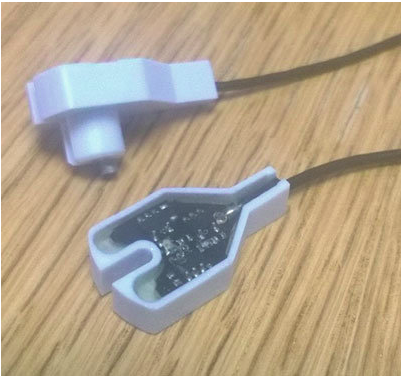
\includegraphics[width=60mm]{{{ImagesSSVEP/dry_active}.png}}}
    \subfigure[]{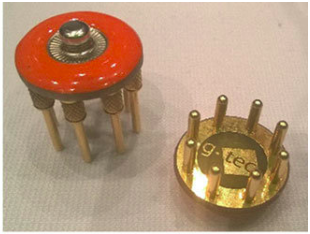
\includegraphics[width=60mm]{{{ImagesSSVEP/gtec_dry}.png}}}
    \caption{(a) Λεπτομέρεια από το εσωτερικό ενός στεγνού και ενεργού ηλεκτροδίου, όπου φαίνεται η πλακέτα του ενισχυτή \cite{Casson2018-fn}. (b) Χαρακτηριστικό παράδειγμα ακιδωτού ηλεκτροδίου από την g.tec, που έρχεται σε επαφή με το δέρμα χωρίς να το διαπερνάει}
    \end{figure}

\end{itemize}
\subsection{Ενίσχυση και Επεξεργασία Σημάτων}
\label{subsec:eeg_amp}
  Τα σήματα που λαμβάνονται από τα ηλεκτρόδια στην επιφάνεια του δέρματος κυμαίνονται μεταξύ $10\mu V$ και $100\mu V$, και πρέπει να ενισχυθούν σημαντικά προκειμένου να γίνει η επεξεργασία τους στα επόμενα στάδια. Το στάδιο της ενίσχυσης περιλαμβάνει αρχικά έναν διαφορικό ενισχυτή με υψηλή απόρριψη κοινού σήματος, και στη συνέχεια δύο η τρία ξεχωριστά στάδια ενίσχυσης με συνολικό κέρδος της τάξης του $10^6$. Επειδή τα σήματα αυτά περιέχουν πολύ θόρυβο σε συχνότητες κοντά στα $0Hz$ (DC συνιστώσα), καθώς και στα $50Hz$ η $60Hz$, λόγω των ηλεκτρομαγνητικών παρεμβολών από ρεύματα τροφοδοσίας στον χώρο. Συνεπώς το σήμα πρέπει να περάσει από διάφορα στάδια υψιπερατού και βαθυπερατού φιλτραρίσματος. Τέλος προκειμένου να σταλθούν τα σήματα στο επόμενο στάδιο της αποθήκευσης και απεικόνισης, γίνεται η χρήση ενός Digital to Analog Converter (DAC). Εδώ φαίνεται και μια από τις χρησιμότητες της ενίσχυσης, καθώς τα DAC δεν μπορούν να λειτουργήσουν με σήματα εισόδου της τάξης των $\mu V$. Τέλος μετά την ψηφιοποίηση του σήματος χρησιμοποιούνται οπτικοί απομονωτές (optical isolator) για λόγους ασφαλείας, έτσι ώστε να μην υπάρχει κίνδυνος να διαρρεύσει ρεύμα από τα επόμενα στάδια (π.χ υπολογιστής), προς τον χρήστη του εγκεφαλογράφου.

\subsection{Μονάδα Αποθήκευσης και Απεικόνισης Σημάτων}
  Αυτό το στάδιο αποτελείται από μια υπολογιστική μονάδα η οποία αποθηκεύει τα σήματα, και χρησιμοποιεί λογισμικό για την απεικόνιση των σημάτων. Επιπλέον σε πολλές περιπτώσεις υπάρχει η δυνατότητα χρήσης επιπλέον τεχνικών επεξεργασίας σε αυτό το στάδιο, όπως χρήση ψηφιακών φίλτρων, κατάτμηση του σήματος σε σημεία ενδιαφέροντος κ.α .
  
  %http://www.braintronics.nl/pages/Productdatabase/Equipment/10BB%20EEG-1042.htm
  %https://www.google.gr/search?q=eeg+recording+device+visualization&source=lnms&tbm=isch&sa=X&ved=0ahUKEwjxxM-q3IrbAhVLMJoKHZsuA98Q_AUICigB&biw=2133&bih=1082#imgrc=aqqrvIP93kudoM:
  \begin{figure}[H]
    \centering     %%% not \center
    \subfigure[]{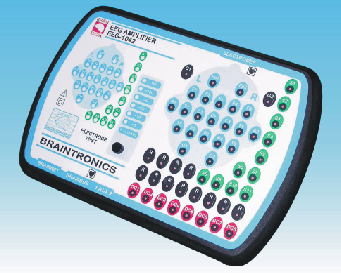
\includegraphics[width=60mm]{{{ImagesSSVEP/amp}.png}}}
    \subfigure[]{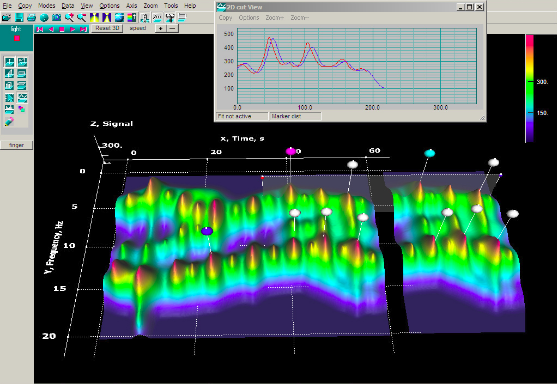
\includegraphics[width=60mm]{{{ImagesSSVEP/eeg_visual}.png}}}
    \caption{(a) Ο ενισχυτής EEG-1142 της Braintronix, με ξεχωριστές αριθμημένες είσοδους για κάθε ηλεκτρόδιο, είναι ένα χαρακτηριστικό παράδειγμα των ενισχυτών που περιγράψαμε στην \ref{subsec:eeg_amp}. (b) Πρόγραμμα απεικόνισης εγκεφαλογραφήματος, καθώς και τρισδιάστασης αναπαράστασης του spectrogram του από την ScienceGL.}
  \end{figure}
\section{Σύστημα 10-20}
Το σύστημα 10-20 χρησιμοποιείται διεθνώς για να περιγράψει και να ορίσει την θέση των ηλεκτροδίων στο κεφάλι. Η χρήση ενός τέτοιου συστήματος είναι απαραίτητη, προκειμένου να υπάρχει ένα κοινό σημείο αναφοράς μεταξύ των ερευνητών για την αναπαραγωγή και σύγκριση των διαφόρων μεθοδολογιών στην εγκεφαλογραφία. Οι αριθμοί $'10'$ και $'20'$ είναι ποσοστά και συμβολίζουν το $10\% $ και $20\% $  της απόστασης μεταξύ των δύο αυτιών, τα οποία με την σειρά τους ορίζουν την απόσταση από ένα αυτί προς το πλησιέστερο σε αυτό ηλεκτρόδιο και την απόσταση μεταξύ δύο γειτονικών ηλεκτροδίων αντίστοιχα.

\par Ανάλογα με την εγκεφαλική περιοχή που καλύπτουν τα ηλεκτρόδια, παίρνουν και το όνομά τους που αποτελείται από ένα γράμμα (η συνδυασμό γραμμάτων) και έναν ζυγό αριθμό για το δεξί ημισφαίριο και περιττό για το αριστερό ημισφαίριο. Ο δείκτης z, προσδιορίζει τα ηλεκτρόδια τα οποία βρίσκονται πάνω στην διαχωριστική γραμμή μεταξύ των δύο ημισφαιρίων. Η βασική διάταξη που αποτελείται από 19 ηλεκτρόδια, είναι η εξής :

\begin{itemize}
    \item Προμετωπιαίος φλοιός (Pre-Frontal cortex) : Fp1, Fp2
    \item Μετωπιαίος λοβός (Frontal lobe) : F3, F4, F7, F8, Fz
    \item Κροταφικός λοβός (Temporal lobe) : T3, T4, T5, T6
    \item Βρεγματικός λοβός (Parietal lobe) : P3, P4, Pz
    \item Ινιακός λοβός (Occipital lobe) : O1, O2
    \item Κεντρική περιοχή (Central) : C3, C4, Cz
\end{itemize}
\begin{figure}[H]
  \centering
  \noindent\makebox[\textwidth]{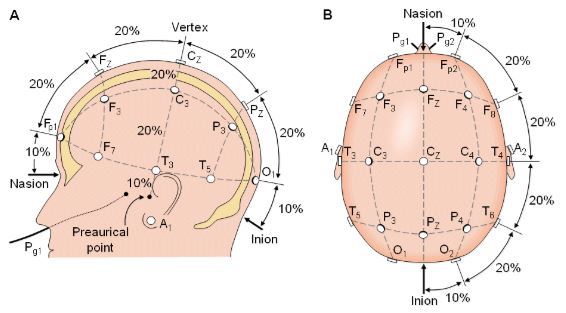
\includegraphics[scale=0.8]{{ImagesSSVEP/10_20}.jpg}}
  \captionsetup{singlelinecheck = false, justification=justified} % used for left alignment
  \caption{Τοποθεσίες ηλεκτροδίων με βάση το σύστημα 10-20. Εικόνα από \cite{Malmivuo1995-jf}. }
  \label{fig:10_20}
\end{figure}
\par Το παραπάνω σύστημα μπορεί να επεκταθεί έτσι ώστε να καλύψει καταστάσεις στις οποίες απαιτείται μεγαλύτερος αριθμός ηλεκτροδίων, ορίζοντας νέες εγκεφαλικές περιοχές μεταξύ αυτών που αναφέρθηκαν, ή και διαφορετικές σχετικές αποστάσεις μεταξύ των ηλεκτροδίων.
\begin{figure}[H]
  \centering
  \noindent\makebox[\textwidth]{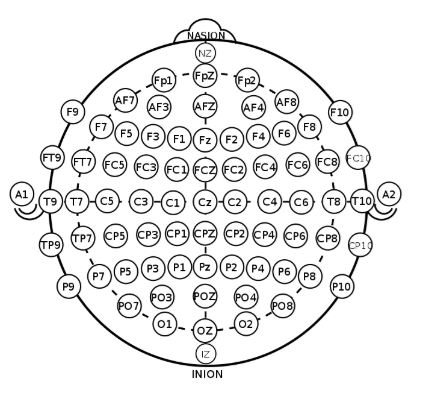
\includegraphics[scale=0.6]{{ImagesSSVEP/10_20_ext}.jpg}}
  \captionsetup{singlelinecheck = false, justification=justified} % used for left alignment
  \caption{Επέκταση συστήματος 10-20. Εικόνα από \cite{Malmivuo1995-jf}. }
  \label{fig:10_20_ext}
\end{figure}

\section{Διεπαφές εγκεφάλου – υπολογιστή (Brain Computer Interfaces)}
  \par Όπως αναφέρθηκε και στην εισαγωγική ενότητα \ref{sec:importance}, οι διεπαφές εγκεφάλου - υπολογιστή (BCIs) εκμεταλλευόμενες την εξέλιξη στις τεχνικές ανάλυσης σημάτων του εγκεφάλου, επιτρέπουν στους χρήστες να επικοινωνούν με το εξωτερικό περιβάλλον χωρίς να απαιτείται οποιαδήποτε μυική κίνηση του χρήστη, μεταφέροντας μηνύματα και εντολές από το μυαλό τους στον υπολογιστή. Στο παρελθόν, η ιδέα ενός BCI το οποίο θα αποκωδικοποιεί τις σκέψεις ενός ατόμου και θα τις μετατρέπει σε εντολές κατανοητές από έναν υπολογιστή, αντιμετωπίστηκε πολύ επιφυλακτικά, ως ένα πολύ περίπλοκο πρόβλημα, λόγω των τεχνικών περιορισμών που υπήρχαν, όπως η χαμηλή χρονική και χωρική ανάλυση καταγραφών, κόστος υλοποίησης real-time εφαρμογών. Σήμερα όμως, η χρήση τέτοιων διεπαφών έχει εξελιχθεί αρκετα και η πληθώρα των υλοποιήσεων έχει οδήγησε στην ανάγκη κατηγοριοποίησης τους. Σύμφωνα με την δημοσίευση \cite{Zander2010-ji} οι διεπαφές εγκεφάλου - υπολογιστή χωρίζονται σε τρεις μεγάλες κατηγορίες : 
  \label{sec:bci_categories}
  \subsection{Active BCIs}
  \par Σε αυτού του είδους τις διεπαφές, ο χρήστης είναι αυτός που συνειδητά προσπαθεί να ελέγξει τα εγκεφαλικά του κύματα, ανεξάρτητα από οποιαδήποτε εξωτερικά ερεθίσματα. Ίσως το πιο αντιπροσωπευτικό δείγμα της κατηγορίας είναι οι διεπαφές οι οποίες βασίζονται στην ανίχνευση κυματομορφών που σχετίζονται με την σκέψη κίνησης ενός μέλους του σώματος, και όχι την πραγματική κίνηση του, γνωστή και στην βιβλιογραφία ως Motor Imagery. Για παράδειγμα, όταν ένας χρήστης σκεφτέι πως κινεί το δεξί του χέρι, το πλάτος των εγκεφαλικών σημάτων στον κινητικό φλοιό αυξάνεται στο δεξί ημισφαίριο και ελαττώνεται στο αρίστερο, και αντίστοιχα για το αριστερό χέρι. Συνήθως για τις διεπαφές αυτής της κατηγορίας απαιτείται μεγάλος χρόνος εκπαίδευσης τόσο του χρήστη, για να ελέγχει και να απομονώνει τις σκέψεις του, όσο και του συστήματος, έτσι ώστε να καταλαβαίνει σωστά τις προθέσεις του χρήστη. 

  \subsection{Reactive BCIs}
  \par Σε αυτήν την κατηγορία ανήκουν οι διεπαφές των οποίων η έξοδος εξαρτάται από εγκεφαλική λειτουργία που προκαλείται ως αντίδραση σε μια εξωτερική διέγερση, η οποία έχει ρυθμιστεί έτσι ώστε να κωδικοποιεί την πρόθεση του χρήστη. Ο χρήστης εξαναγκάζει τα εγκεφαλικά του σήματα να παραμένουν σε μια συγκεκριμένη κατάσταση, απλά με το να παρατηρεί η να συγκεντρώνεται σε μια συγκεκριμένη εξωτερική διέγερση. Το πλεονέκτημα αυτών των διεπαφών είναι πως τα προκαλούμενα σήματα είναι παρόμοια από χρήστη σε χρήστη, και πως απαιτείται ελάχιστη η καθόλου εκπαίδευση για να λειτουργήσουν.

  \subsection{Passive BCIs}
  \par Τέλος, σε αυτού του τύπου τις διεπαφές, ο χρήστης δεν έχει άμεσο έλεγχο του αποτελέσματος καθώς δεν απαιτείται προσπάθεια απο τον χρήστη να ελέγξει τα εγκεφαλικά του σήματα. Αντί αυτού, η έξοδος του συστήματος επηρεάζεται από την νοητική κατάσταση του χρήστη, όπως για παράδειγμα τα επίπεδα προσοχής του, τα συναισθήματα του ή τα επίπεδα κόπωσης. Πολλές φορές σε αυτού του είδους τις διεπαφές η έξοδος τους γίνεται γνωστή στον χρήστη μέσω κάποιας ηχιτικής ή οπτικής ένδειξης, επηρεάζοντας εκ νέου την νοητική του κατάσταση, και δημιουργώντας ένα είδος ανάδρασης (neuro-feedback). 
  
  \par Παρότι η παραπάνω κατηγοριοποίηση δίνει μια σαφή εικόνα όλων των διαφορετικών BCIs, υπάρχουν περιπτώσεις όπου τα όρια μεταξύ των παραπάνω ορισμών δεν είναι απολύτως σαφή. Για παράδειγμα, στην περίπτωση της neuro-feedback ανάδρασης, ο χρήστης είναι πολύ πιθανόν να προσπαθήσει να αλλάξει την νοητική του κατάσταση επηρεαζόμενος από την έξοδο της διεπαφής, μετατρέποντας έτσι το είδος του BCI από passive σε active. Ακόμα όμως και στην περίπτωση των active διεπαφών, η πρόθεση του χρήστη για το τι εγκεφαλικά σήματα θα παράξει, επηρεάζεται από το αποτέλεσμα της προηγούμενης πρόθεσης του, το οποίο μπορεί να θεωρηθεί ως εξωτερική διέγερση, συνεπώς καταλήγουμε σε τύπο reactive. 

  \subsection{Κριτήρια Αξιολόγησης Απόδοσης των BCIs}
  \subsubsection{ITR}
  \subsubsection{Accuracy}
  
\section{Χαρακτηριστικά Εγκεφαλικά σήματα}
  \par Σε αυτό το σημείο θα αναφερθούμε σε κάποια βασικά εγκεφαλικά σήματα που παράγονται στον εγκέφαλο, είτε ακούσια είτε εκούσια, και τα οποία χρησιμοποιούνται για την υλοποίηση των διαφόρων τύπων BCIs που αναφέρθηκαν στην ενότητα \ref{sec:bci_categories}. Γενικά, τα EEG σήματα ταξινομούνται με κριτήριο την συχνότητά, το πλάτος, την μορφή, καθώς και την τοποθεσία στο κρανίο όπου καταγράφονται.
  
  \subsection{Εγκεφαλικοί ρυθμοί}
    \par Αυτού του είδους τα σήματα εμφανίζονται φυσιολογικά σε όλους του εγκεφάλους, ταξινομούνται με κριτήριο την συχνότητα τους, και η παρουσία τους ή η απουσία τους, βοηθάει την εξαγωγή συμπερασμάτων όσον αφορά τόσο την νοητική κατάσταση του χρήστη, όσο και την ύπαρξη κάποια νευρολογικής ασθένειας. Τα σχόλια που ακολουθούν για καθέναν από τους ρυθμούς αυτούς αφορούν υγιής ενήλικες οργανισμούς, καθώς στην αντίθετη περίπτωση υπάρχουν αρκετές διαφοροποιήσεις, το οποίο σημαίνει πως οι ρυθμοί αυτοί μπορούν να χρησιμοποιηθούν και για την διάγνωση ασθενειών. 
    \begin{itemize}
        \item {Κύματα Δέλτα}
        \par Κύματα Δέλτα ονομάζουμε τις συχνότητες με εύρος $0.5 - 4 Hz$ και εμφανίζονται κυρίως σε νεογνά και ενήλικες κατά την διάρκεια του ύπνου (deep stage 3 of NREM), και ίσως εμπλέκονται στην διαδικασία σχηματισμού της μνήμης \cite{Maquet2001-cs}
        \item {Κύματα Θήτα}
        \par Κύματα Θήτα ονομάζονται οι κυματομορφές με εύρος συχνοτήτων $4 - 8Hz$ και σε φυσιολογικούς ενήλικες εμφανίζονται σε πολύ μικρή ποσότητα, και συχνά όταν κάποιος βρίσκεται στην κατάσταση της ονειροπόλησης (daydreaming)
        \item {Κύματα Άλφα}
        \label{item:alpha}
        \par Τα κύματα Άλφα, τα οποία ήταν τα πρώτα κύματα που ανιχνεύτηκαν στον εγκέφαλο από τον Hans Berger \cite{Berger1933-pg}, και κυμαίνονται μεταξύ $8 - 13Hz$. Κυρίως εμφανίζονται στον οπτικό φλοιό κατά την διάρκεια της ξεκούρασης με κλειστά μάτια, όχι όμως σε κατάσταση ύπνου, όπου τότε ελαττώνονται. 
        \item {Κύματα Βήτα}
        \par Τα κύματα Βήτα ανακαλύφθηκαν και αυτά από τον Hans Berger, αμέσως μετά τα Άλφα, και η συχνότητα τους κυμαίνεται μεταξύ $13 - 30Hz$. Εμφανίζονται όταν το άτομο έχει ανοιχτά μάτια, και βρίσκεται σε κατάσταση συγκέντρωσης, όταν προσπαθεί να λύσει ένα πρόβλημα ή και σε καταστάσεις άγχους.
        \item{Κύματα Γάμμα}
        \par Το εύρος συχνοτήτων των κυμάτων Γάμμα είναι μεταξύ $30 - 80Hz$, και όπως και τα Βήτα, εντοπίζονται στον εγκέφαλο σε καταστάσεις έντονης εγρήγορσης \cite{Bressler1990-im}. Παρόλαυτα έχουν καταγραφεί και κατά τις φάσεις του REM ύπνου, κατά την οποία δεν υπάρχει συνείδηση και εγρήγορση στο άτομο \cite{Steriade1996-pg}.
    \end{itemize}

    \begin{figure}[H]
        \centering
        \noindent\makebox[\textwidth]{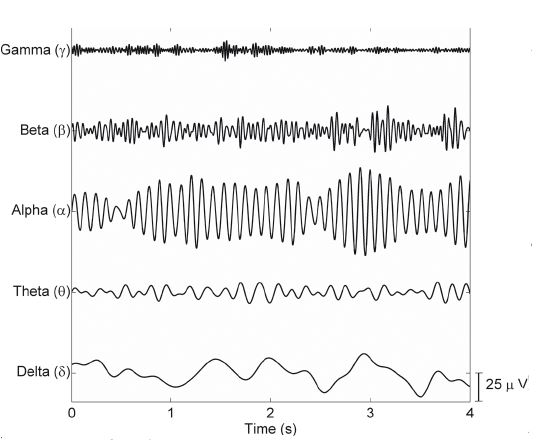
\includegraphics[scale=0.7]{{ImagesSSVEP/eeg_waves}.jpg}}
        \captionsetup{singlelinecheck = false, justification=justified} % used for left alignment
        \caption{Γραφική αναπαράσταση των φυσιολογικών κυματομορφών του εγκεφάλου. Εικόνα από \cite{Scarano2012-ok}}
        \label{fig:eeg_waves}
    \end{figure}
    %πως χρησιμοποιούνται σε BCI / efarmoges
  \subsection{Προκλητά Δυναμικά (ΠΔ)}  
    \par Ως προκλητά δυναμικά, ορίζονται οι διαφορές δυναμικού στο εγκεφαλικό σήμα που ανιχνεύονται σε συγκεκριμένο χρονικό διάστημα, ως αντίδραση σε ένα εξωτερικό ερέθισμα. Τα δυναμικά αυτά παρουσιάζουν μεγάλο ερευνητικό ενδιαφέρον και χρησιμοποιούνται κατά κόρον, τόσο για την διάγνωση ασθενειών του εγκεφάλου και των νεύρων, όσο και για την υλοποίηση BCIs.  Ένας λόγος που χρησιμοποιούνται ευρέως σε BCIs, είναι πως τα προκλητά δυναμικά μπορούν να αναπαραχθούν κατά βούληση,  κατά την διάρκεια πειραμάτων στα οποία παρέχουμε την κατάλληλη διέγερση, συνεπώς είναι πιο εύκολη η μελέτη τους για την χρήση τους σε διεπαφές εγκεφάλου - υπολογιστή, συγκριτικά με άλλα εγκεφαλικά σήματα όπως η φυσιολογικοί εγκεφαλικοί ρυθμοί, που εξαρτώνται από την ψυχολογία και την κατάσταση του ατόμου.
    Τα ΠΔ χωρίζονται σε δύο μεγάλες κατηγορίες, τα ενδογενή και τα εξωγενή δυναμικά \cite{Sutton1965-nl}.  Τα εξωγενή δυναμικά σχετίζονται άμεσα με τα χαρακτηριστικά του εξωτερικού ερεθίσματος (π.χ ένταση, συχνότητα), ενώ τα ενδογενή δυναμικά σχετίζονται με την ψυχολογική αντίδραση του ατόμου στο εξωτερικό ερέθισμα. Στη συνέχεια θα αναφερθούμε στα πιο γνωστά σήματα κάθε κατηγορίας. Τέλος αξίζει να αναφερθεί πως για κάθε μια από αυτές τις κατηγορίες, τα ερεθίσματα μπορούν να είναι διαφόρων ειδών, όπως οπτικά, ακουστικά, σωματικά κ.α.
    \subsubsection{Ενδογενή ΠΔ - P300}  
      \paragraph{Περιγραφή} ~\\
      \par Το ενδογενές δυναμικό που κυριαρχεί τόσο στην έρευνα όσο και στην χρήση του σε BCIs, είναι το P300 \cite{Gordeev2007-pu}. Αποτελείται από μια θετική διακύμανση στην τάση, η οποία κατά μέσο όρο προκύπτει 300ms αφότου εμφανιστεί το ερέθισμα. Το πλάτος της διακύμανσης κυμαίνεται περίπου από 30μV στην περιοχή του εγκεφάλου που καλύπτεται από το ηλεκτρόδιο Pz, ενώ αρκετά χαμηλότερο πλάτος, κοντά στα 5μV, στην περιοχή Fz \cite{Perlman2013-sg}. Προκειμένου να προκληθούν σήματα P300, το άτομο πρέπει να συγκεντρώνει την προσοχή του σε σπανίως εμφανιζόμενα ερεθίσματα (target), τοποθετημένα τυχαία ανάμεσα σε μια σειρά από συχνά εμφανιζόμενα ερεθίσματα (non target). Αυτή η διαδικασία είναι γνωστή στην ξένη βιβλιογραφία ως “oddball paradigm”. Υπάρχουν αρκετοί λόγοι που καθιστούν τα P300 τόσο δημοφιλή. Αρχικά, τα P300 είναι σήματα τα οποία μπορούν να δημιουργηθούν στον εγκέφαλο του καθενός, χωρίς να απαιτείται σχεδόν καθόλου εκπαίδευση από τον χρήστη. Επιπλέον, είναι εύκολα ανιχνεύσιμα, και αρκετά συνεπή όσον αφορά τον χρόνο που θα εμφανιστούν μετά το κατάλληλο ερέθισμα \cite{Fazel-Rezai2012-mk}. 
      
      \paragraph{Εφαρμογές} ~\\
      \par Ίσως η πιο διάσημη εφαρμογή των P300 είναι σε συστήματα BCI, και συγκεκριμένα σε μηχανές συλλαβισμού (spellers). Πρώτοι οι  Farwell και  Donchin περιέγραψαν και υλοποίησαν μια τέτοια μηχανή \cite{Farwell1988TalkingPotentials} Η διαδικασία που ακολουθήθηκε είναι η εξής. Αρχικά δημιουργήθηκε ένα γραφικό περιβάλλον, που παράγει τα οπτικά ερεθίσματα που θα προκαλέσουν τα P300, και αποτελείται από ένα πίνακα 6x6 με αλφαριθμητικούς χαρακτήρες. Κάθε γραμμή και στήλη του πίνακα, ακολουθεί ένα μοτίβο που αποτελείται από 100ms κατά τα οποία όλα τα στοιχεία της κάθε γραμμής ή στήλης έχουν υψηλή φωτεινότητα, και 80ms χαμηλή. Το μοτίβο αυτό συμβαίνει διαδοχικά σε κάθε γραμμή ή στήλη, και με τυχαία σειρά. Συνεπώς δημιουργείται μια ακολουθία 12 τέτοια μοτίβα. Ο χρήστης κάθε φορά είναι συγκεντρωμένος σε ένα συγκεκριμένο αλφαριθμητικό, το οποίο ταυτόχρονα ανήκει σε μια γραμμή και μια στήλη, που αποτελούν τα target ερεθίσματα, σε αντίθεση με τα non-target που αποτελούνται από τις άλλες 10 στήλες και γραμμές. Ανιχνεύοντας λοιπόν τα P300 σήματα που παράγονται, είναι δυνατόν να παρθεί απόφαση για το αλφαριθμητικό στο οποίο είχε συγκεντρωθεί ο χρήστης. Το ποσοστό επιτυχίας που σημείωσαν οι χρήστες ήταν $95\%$ με ταχύτητα 1 χαρακτήρα κάθε 26 δευτερόλεπτα.
      \begin{figure}[H]
        \centering
        \noindent\makebox[\textwidth]{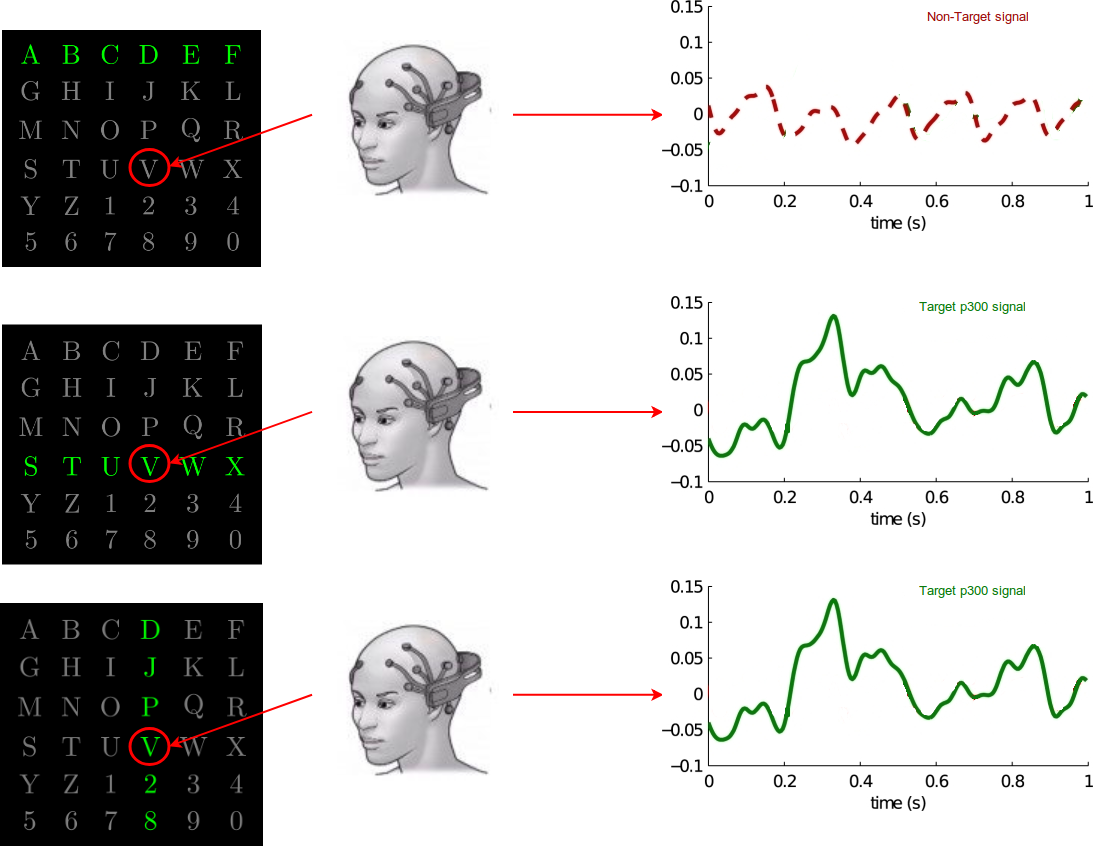
\includegraphics[scale=0.3]{{ImagesSSVEP/p300_speller}.png}}
        \captionsetup{singlelinecheck = false, justification=justified} % used for left alignment
        \caption{Παράδειγμα διέπαφης βασισμένης στα P300 σήματα, για την υλοποίηση μηχανής συλλαβισμού. Ο χρήστης συγκεντρώνεται στο επιθυμητό γράμμα (V), και παράγονται P300 σήματα, όταν φωτιστεί η γραμμή και η στήλη που το περιέχουν.}
        \label{fig:p300_speller}
      \end{figure}

    \subsubsection{Εξωγενή ΠΔ - SSVEP}  
      \paragraph{Περιγραφή} ~\\
      \par Συνήθως τα εξωγενή προκλητά δυναμικά παράγονται από ένα διακριτό ερέθισμα, απομονομένο χρονικά από άλλα πιθανά ερεθίσματα. Ωστόσο, είναι δυνατή η παραγωγή δυναμικών στον εγκέφαλο, προκαλούμενα απο μια ακολουθία διεγέρσεων (impulse train), οι οποίες εμφανίζονται διαδοχικά με σταθερή συχνότητα. Επειδή η απόκριση σε μια τέτοια ακολουθία οπτικών διεγέρσεων είναι σχετικά σταθερή σε πλάτος, φάση, ονομάστηκαν το 1966 από τον Regan \cite{Regan1966-gn}, οπτικά προκλητά δυναμικά σταθερής κατάστασης, ή αλλιώς Steady State Visual Evoked Potentials (SSVEP). Ωστόσο η ανακάλυψη αυτών των δυναμικών φαίνεται να έγινε πρώτη φορά το 1935, από τους Adrian και Matthews \cite{1935-sw}, χωρίς όμως να τους δώσουν κάποια συγκεκριμένη ονομασία. 
      \par Η σημαντική λεπτομέρεια που καθιστά τα SSVEP τόσο χρήσιμα στην υλοποίηση διεπαφών εγκεφάλου - υπολογιστή, είναι πως η συχνότητα της προκαλούμενης κυματομορφής στον εγκέφαλο, συμπίπτει με την συχνότητα των οπτικών παλμών της διέγερσης. Με αυτόν τον τρόπο, δημιουργώντας οπτικές πηγές που εκπέμπουν παλμούς σε διαφορετικές συχνότητες, μπορούμε να αντιστοιχίσουμε κάποιες επιθυμητές εντολές σε κάθε μία από αυτές, και συνεπώς μέσω ανάλυσης των παραγόμενων SSVEP σημάτων, να ανιχνεύεται η φωτεινή πηγή στην οποία είναι συγκεντρωμένος ο χρήστης, δηλαδή η εντολή την οποία θέλει να πραγματοποιήσει.  

       \begin{figure}[H]
        \centering                                      
        \noindent\makebox[\textwidth]{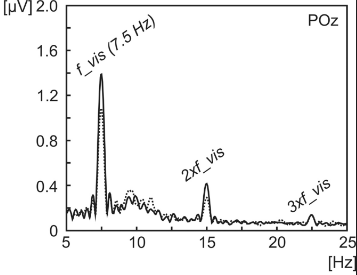
\includegraphics[scale=0.6]{{ImagesSSVEP/ssvep_example}.png}}
        \captionsetup{singlelinecheck = false, justification=justified} % used for left alignment
        \caption{SSVEP σήματα που παράχθηκαν ώς αντίδραση στον εστιασμό των ματιών σε φωτεινή διέγερση συχνότητας $7.5Hz$. Παρατηρούμε πως εκτός από την κύρια συνιστώσα, έχουμε έντονες κορυφές και στις αρμονικές συχνότητες, δηλαδή $15Hz$ και $22.5Hz$. Εικόνα απο \cite{Saupe2009-wn}}
        \label{fig:ssvep_example}
    \end{figure}
    
      \par Το σημείο του εγκεφάλου που παράγονται τα SSVEP σήματα βρίσκεται στον ινιακό φλοιό (occipital lobe), το οποίο είναι λογικό αν σκεφτούμε πως εκέι βρίσκεται το κέντρο επεξεργασίας της όρασης στον εγκέφαλο. Στο απλό σύστημα 10-20 υπάρχουν μόνο δύο ηλεκτρόδια που καλύπτουν τον φλοιό, τα  Ο1 και Ο2, ένω στις επαυξημένες εκδοχές του συστήματος, βρίσκουμε επιπλέον και τα ηλεκτρόδια, Oz που βρίσκεται ανάμεσα στα Ο1 και Ο2, καθώς και τα PO3, PO7, POz, P04, P08, που καλύπτουν τα σύνορα μεταξύ ινιακού και βρεγματικού λοβού. Στις περισσότερες μελέτες χρησιμοποιείται διάφοροι πιθανοί συνδυασμοί των παραπάνω ηλεκτροδίων, η και όλα. Ωστόσο η καλύτερη ποιότητα SSVEP σήματος, φαίνεται να εμφανίζεται στα O2 και Oz \cite{Oikonomou2016-te}.
    \begin{figure}[H]
        \centering                                      
        \noindent\makebox[\textwidth]{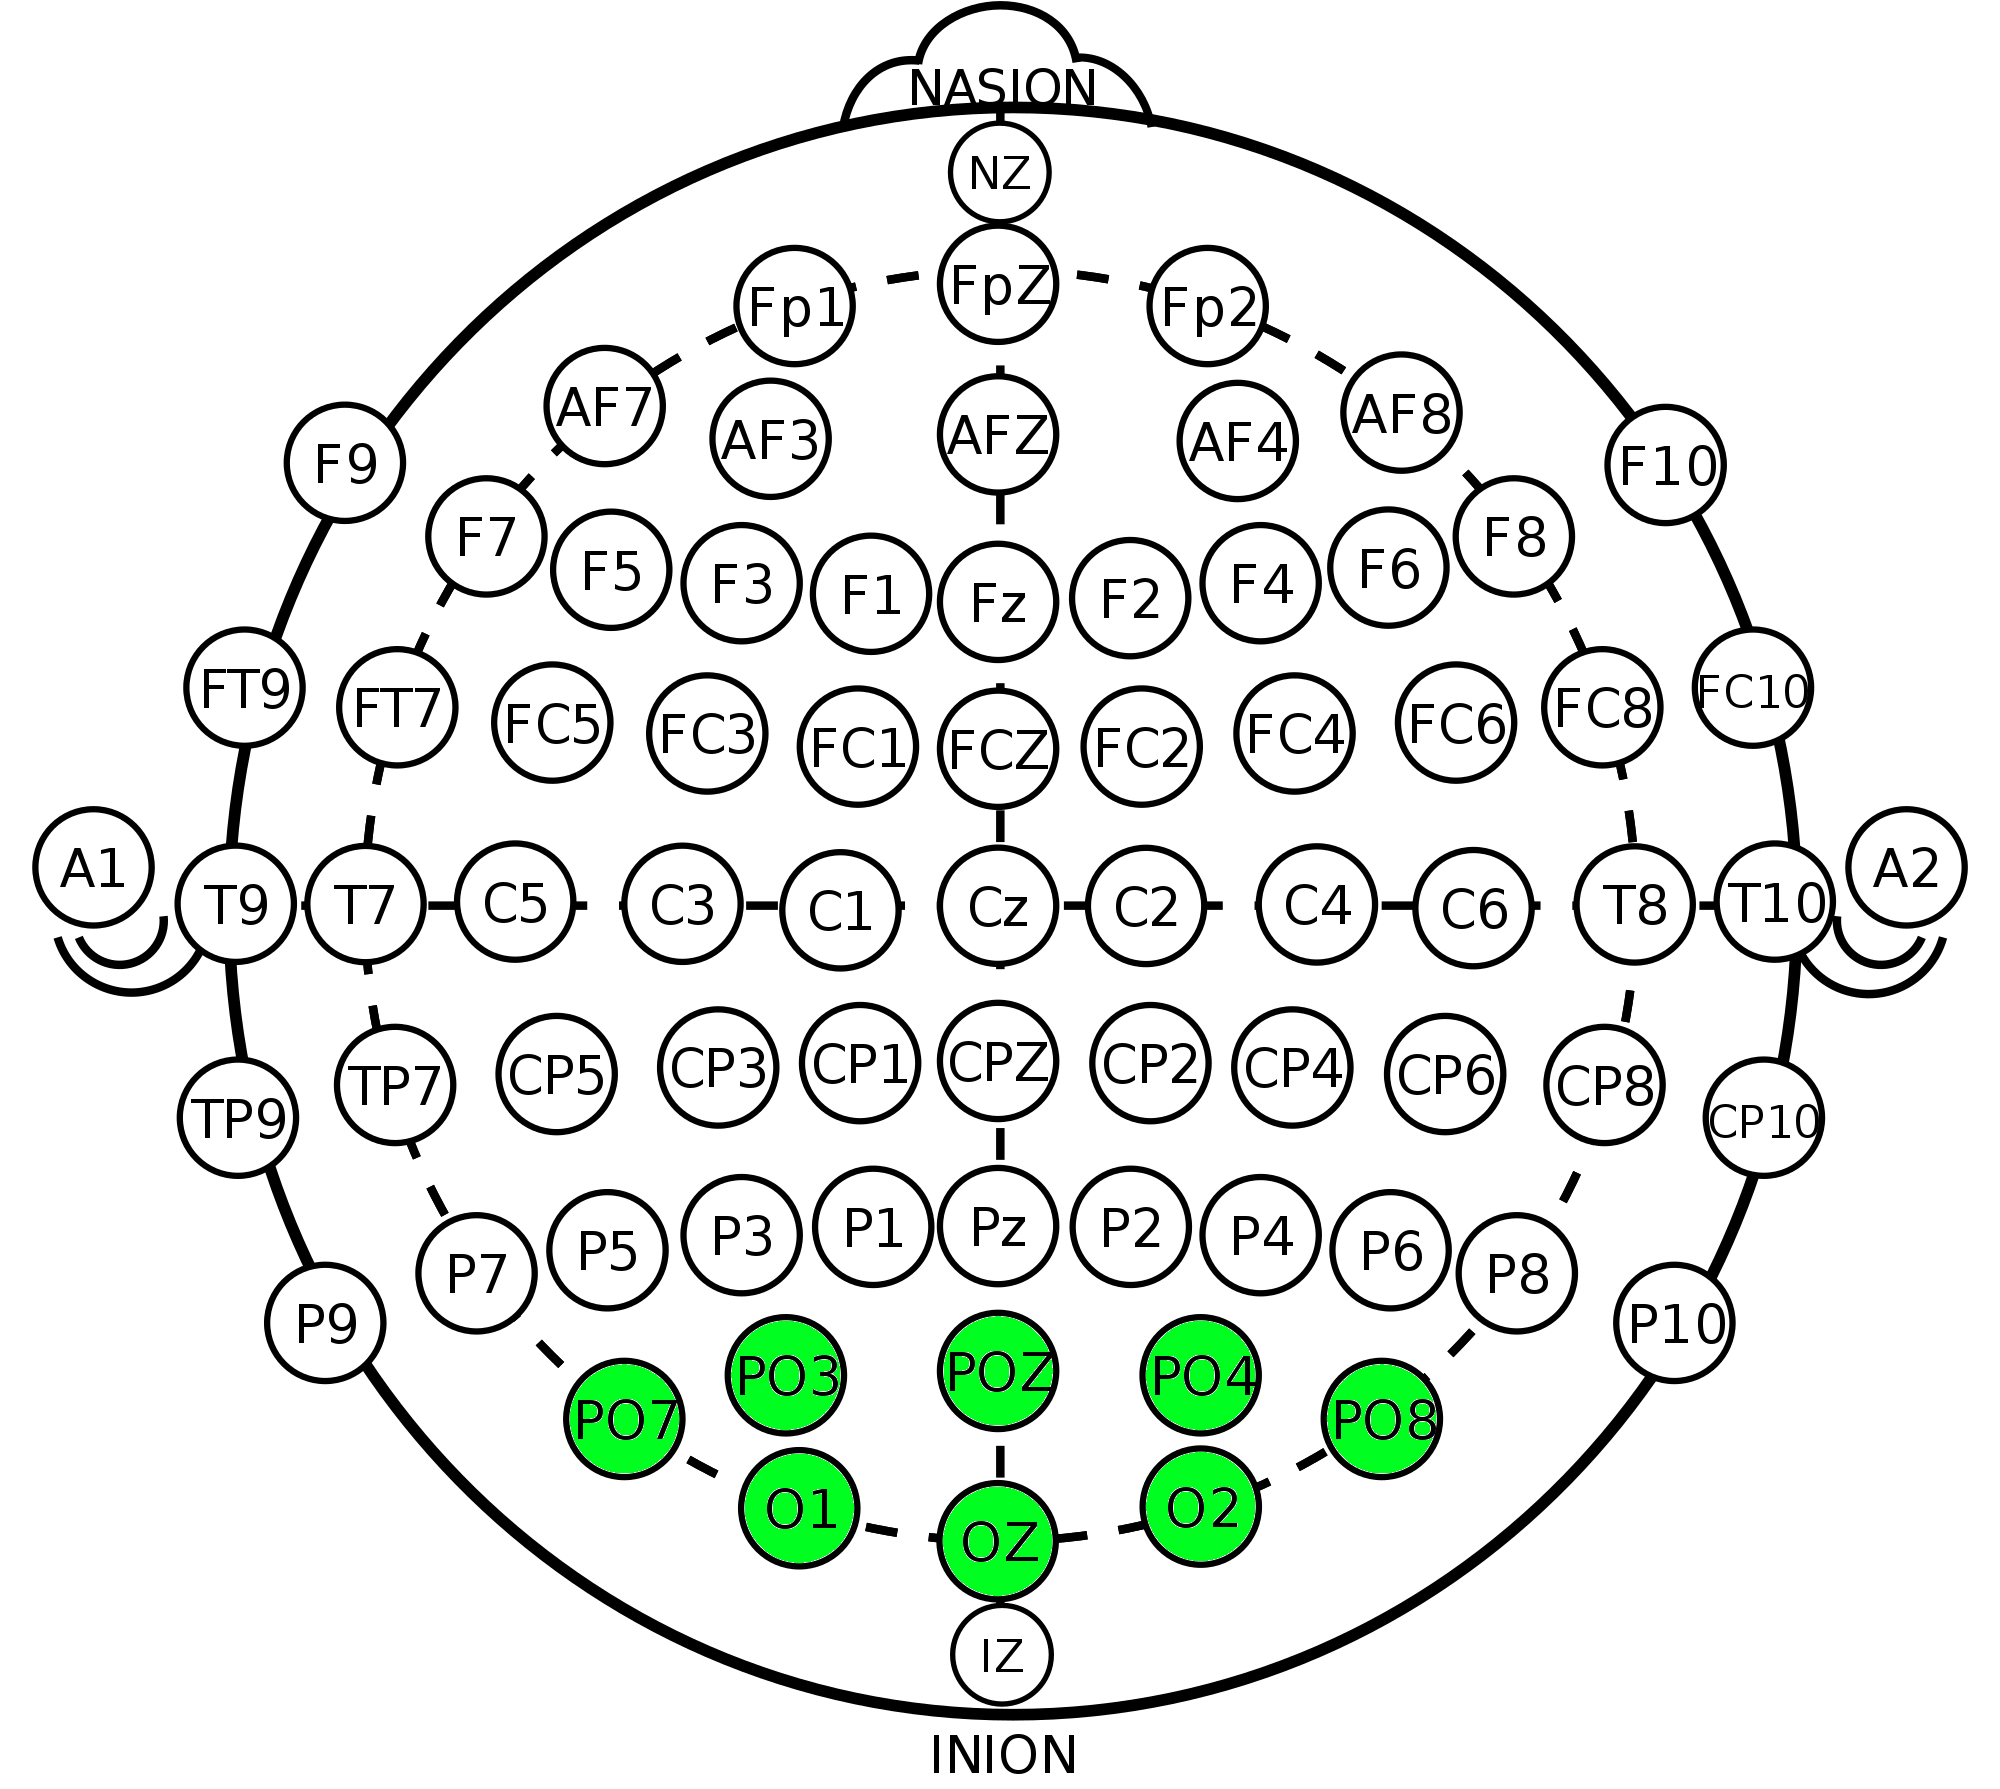
\includegraphics[scale=0.1]{{ImagesSSVEP/occ_electrodes}.png}}
        \captionsetup{singlelinecheck = false, justification=justified} % used for left alignment
        \caption{Ηλεκτρόδια που καλύπτουν τον ινιακό λοβό και την γύρω περιοχή, και στα οποία εμφανίζονται τα SSVEP σήματα.}
        \label{fig:occ_electrodes}
    \end{figure}
    
    \paragraph{Επιλογή Συχνοτήτων των Οπτικών Διεγέρσεων} ~\\
      \label{par:freq_choose}
      \par Προκειμένου να προκληθούν SSVEP, η συχνότητα της διέγερσης πρέπει να ανήκει στο εύρος $3.5 - 75Hz$. Συνήθως χωρίζουμε το εύρος αυτό σε 3 περιοχές, τα εύρη των οποίων όμως ορίζονται διαφορετικά από μελέτη σε μελέτη. Σύμφωνα με τον Regan \cite{regan1989human} έχουμε: Χαμηλές συχνότητες $1 - 12Hz$, Μεσαίες συχνότητες $12 - 30Hz$, και Υψηλές συχνότητες $30 - 60Hz$. Ένα από τα σημαντικότερα ερωτήματα, είναι το πώς μπορούμε να επιλέξουμε εκείνες τις συχνότητες που θα αποφέρουν μέγιστη απόδοση στο σύστημά μας. Η μεγάλη ποικιλία των συχνοτήτων που χρησιμοποιούνται στην βιβλιογραφία, είναι σημάδι πως αυτό το ερώτημα είναι ακόμα αναπάντητο. Ενδεικτικά, στην βιβλιογραφική δημοσίευση \cite{zhu2010survey}, μελετήθηκε το είδος των διεγέρσεων που χρησιμοποιήθηκαν σε 57 διαφορετικές ερευνητικές εργασίες, όπου συνολικά υπήρξαν 35 διαφορετικοί συνδυασμοί συχνοτήτων. Επιπλέον, στην ίδια εργασία, αναφέρεται πως σε 49 εργασίες χρησιμοποιήθηκαν συχνότητες που άνηκαν στην χαμηλή ζώνη. 
      \par Η χρήση χαμηλο-μεσαίων συχνοτήτων υποστηρίζεται από το γεγονός πως τα παραγόμενα SSVEP έχουν καλό σηματο-θορυβικό λόγο (SNR) και μπορούν να παραχθούν εύκολα \cite{yijun2005brain}. Ωστόσο παρουσιάζουν και σημαντικά μειονεκτήματα. Η εστίαση της προσοχής σε πηγές φωτός που πάλλονται σε χαμηλές συχνότητες μπορεί να προκαλέσει κούραση (fatigue) του ματιού \cite{lin2012snr}, ημικρανίες. \cite{detommaso1999steady}, ακόμα και επιληπτικές κρίσεις \cite{lin2012snr}. Τέλος ένας άλλος σημαντικός λόγος, είναι πως η περιοχή αυτών των συχνοτήτων περιλαμβάνει τις συχνότητες όπου εμφανίζονται τα κύματα Άλφα \ref{item:alpha}, τα οποία είναι τα πιο συχνά εμφανιζόμενα κύματα στον ανρθώπινο εγκέφαλο, προκαλώντας την παραγωγή πολλών false positive, δηλαδή την ανίχνευση SSVEP σημάτων, χωρίς να υπάρχουν πραγματικά. Αντιθέτως η χρήση υψηλών συχνοτήτων, προκαλεί λιγότερη κούραση στο μάτι, χωρίς τον κίνδυνο επιληπτικών κρίσεων και με σαφώς λιγότερα false positives. Το πλάτος των παραγόμενων SSVEP σημάτων ελαττώνεται με την αύξηση της συχνότητας διέγερσης, χωρίς όμως να ελαττώνεται με τον ίδιο ρυθμό ο SNR, καθώς στις υψηλές συχνότητες, ελαττώνεται και ο θόρυβος λόγω μειωμένης εγκεφαλικής δραστηριότητας \cite{wang2006practical}. 
      
      \par Ανεξαρτήτως ποιας ζώνης οι συχνότητες θα επιλεγούν για την υλοποίηση μιας τέτοιας διεπαφής, πρέπει να ληφθεί ιδιαίτερη προσοχή έτσι ώστε καμία συχνότητα να μην είναι ακέραιο πολλαπλάσιο κάποιας άλλης, δηλαδή να μην είναι αρμονική συχνότητα. Ο λόγος είναι πως μια συγκεκριμένη συχνότητα διέγερσης, παράγει SSVEP σήματα τόσο σε αυτήν την συχνότητα όσο και στις αρμονικές τις, όπως φαίνεται και στην εικόνα \ref{fig:ssvep_example}. Για παράδειγμα, στην περίπτωση διεπαφής με δύο οπτικές διεγέρσεις, μία στα $10Hz$ και μία στα $20Hz$, η ανίχνευση της συχνότητας $20Hz$ στο SSVEP σήμα, θα μπορούσε να προκληθεί είτε ο χρήστης κοίταγε την διέγερση των $10Hz$ είτε των $20Hz$.
    
      \begin{figure}[H]
        \centering                                      
        \noindent\makebox[\textwidth]{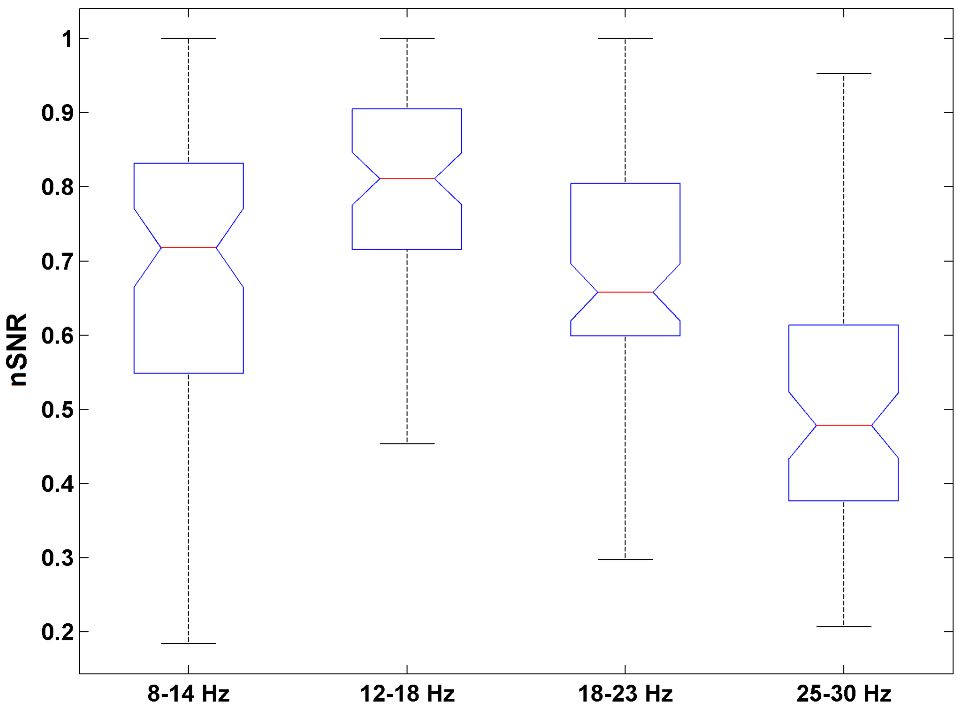
\includegraphics[width = 80mm]{{ImagesSSVEP/snr}.JPG}}
        \captionsetup{singlelinecheck = false, justification=justified} % used for left alignment
        \caption{Κατανομή SNR σε κάθε συχνοτική περιοχή, όπου η κόκκινη γραμμή αναπαριστά την ενδιάμεση τιμή των μετρήσεων για 10 διαφορετικά άτομα. Εικόνα από \cite{kus2013quantification}}
        \label{fig:occ_electrodes}
      \end{figure}
    
      
      %ΔΗΜΟΓΡΑΦΙΚΑ ΠΟΙΟΙ ΜΠΟΡΟΥΝ
      \paragraph{Τύπος Οπτικής Διέγερσης} ~\\
      \label{subsec:visual_stimulus}  
      \par Ένας ακόμα σημαντικός παράγοντας που μαζί με την κατάλληλη επιλογή συχνοτήτων επηρεάζουν πιο πολύ την ποιότητα του σήματος,  είναι το είδος της συσκευής που θα χρησιμοποιηθεί για να επιτευχθεί η επαναλαμβανόμενη διέγερση \cite{wu2008stimulator}. Κάνοντας μια ανασκόπηση στην βιβλιογραφία παρατηρούμε πως υπάρχουν 3 βασικοί τρόποι επίτευξης της επαναλαμβανόμενης οπτικής διέγερσης (ΕΟΔ) \cite{zhu2010survey} : 
      
      \begin{itemize}
        \item {Πηγές Φωτός}
        \par Τέτοιου είδους οπτικές διεγέρσεις δημιουργούνται κάνοντας χρήση φωτεινών πηγών όπως Light Emiting Diodes (LEDs), λαμπτήρων φθορισμού, ή λαμπτήρων με Ξένο (Xe). Στην πλειοψηφία των περιπτώσεων, απαιτείται ξεχωριστό κύκλωμα οδήγησης το οποίο παρέχει και τους κατάλληλους παλμούς για την διαμόρφωση της κατάλληλης συχνότητας. H πρώτη διεπαφή SSVEP το 1996 \cite{Calhoun1996-ei}, χρησιμοποιούσε Λαμπτήρες φθορισμού, ωστόσο πλέον τα LEDs κυριαρχούν. Ενδεικτικά, στην ίδια βιβλιογραφική δημοσίευση \cite{zhu2010survey} που αναφέρθηκε στην προηγούμενη παράγραφο, 24 από τις 58 εργασίες χρησιμοποίησαν LEDs διαφόρων χρωμάτων.
        \item {Μονά Μοτίβα σε Οθόνη}
        \par Τα μοτίβα αυτά συνήθως είναι δισδιάστατα σχήματα (παραλληλόγραμμα, βελάκια κ.α) τα οποία δημιουργούνται σε οθόνες, και η συχνότητα διαμόρφωσης αυτής της διέγερσης καθορίζονται από τους χρόνους που εμφανίζονται και εξαφανίζονται από την οθόνη.
        \item {Διπλά Μοτίβα σε Οθόνη}
        \par Σε αυτή την κατηγορία υπάρχουν 2 διαφορετικά μοτίβα-σχήματα, συμπληρωματικά μεταξύ τους, τα οποία εναλλάσσονται. Η βασική διαφορά με την προηγούμενη κατηγορία, είναι πως ενώ στην περίπτωση του ενός σχήματος, η συχνότητα της οπτικής διέγερσης (2 εναλλαγές μεταξύ των μοτίβων) προκαλεί SSVEP σήματα στην ίδια συχνότητα, αυτή η κατηγορία προκαλεί SSVEP στην διπλάσια συχνότητα.
    \end{itemize}
    \par  
    
    \begin{figure}[H]
    \centering     %%% not \center
    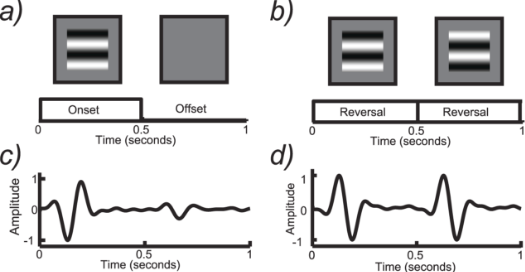
\includegraphics[width=100mm]{{{ImagesSSVEP/patern_reversal}.png}}
    %\subfigure[]{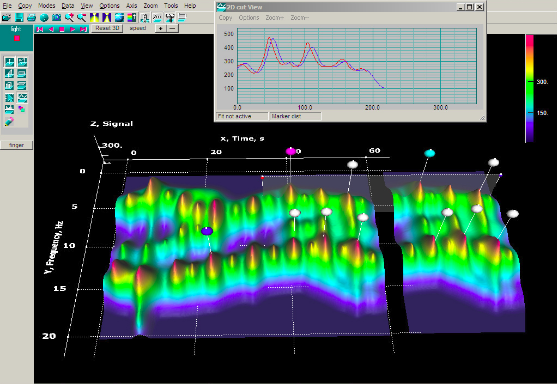
\includegraphics[width=60mm]{{{ImagesSSVEP/eeg_visual}.png}}}
    \caption{Παράδειγμα ενός πλήρη κύκλου οπτικής διέγερσης για την περίπτωση μονών (a) και διπλών συμπληρωματικών (b) μοτίβων, καθώς και η μορφή των παραγόμενων SSVEPs, στα οποία φαίνεται πως για ίδια συχνότητα διέγερσης τα διπλά μοτίβα προκαλούν SSVEPs διπλάσιας συχνότητας. Εικόνα από \cite{Norcia2015-bi}}
  \end{figure}
  
    %πες και για επιλογη χρώματος οπτικής διέγερσης - ισως στο 4ο κεφαλαιο.

\end{document}
 % EEG Background Theory

\lhead{\emph{Κεφάλαιο 3}}

%% !TEX root = ../Thesis.tex
%% !TEX output_directory
\documentclass[11pt,a4paper,english,greek,twoside]{../Thesis}
\usepackage{mathtools}  
\mathtoolsset{showonlyrefs}  
\begin{document}
%\everymath{\displaystyle}
\chapter{Θεωρητικό υπόβαθρο}\label{chap:Background}
\par Σε αυτό το κεφάλαιο θα παρουσιαστούν όλες οι υπολογιστικές μέθοδοι που χρησιμοποιήθηκαν σε αυτήν την διπλωματική εργασία, και που αφορούν την προ-επεξεργασία των εγκεφαλικών σημάτων, την εξαγωγή κατάλληλων-αντιπροσωπευτικών χαρακτηριστικών από τα σήματα, τα οποία θα χρησιμοποιηθούν ως είσοδος στους αλγορίθμους απόφασης και μηχανικής μάθησης. Σε αυτό το επίπεδο θα γίνει μόνο μια αναφορά στα γενικά χαρακτηριστικά της κάθε μεθόδου, οπότε είναι πιθανό να μην γίνει άμεσα αντιληπτός ο συγκεκριμένος τρόπος με τον οποίον θα εφαρμοστεί η κάθε μέθοδος στο παρών πρόβλημα. Αυτού του είδους η ανάλυση θα γίνει στις υποενότητες \ref{subsec:preprocessing} και \ref{subsec:featureExtract}
\section{Αποθορυβοποίηση - Φιλτράρισμα}
\subsection{Είδη Φίλτρων}
Γενικά η λειτουργία ενός φίλτρου μπορεί να χαρακτηριστεί από τη χαρακτηριστική του απόκριση στο πεδίο του χρόνου. Πιο συγκεκριμένα, οι πιο συχνά χρησιμοποιούμενες κατηγορίες αφορούν φίλτρα τα οποία επιτρέπουν την διέλευση συχνοτήτων από ένα κατώφλι και άνω, όπου ονομάζονται υψιπερατά, ενώ από ένα κατώφλι και κάτω, βαθυπερατά. Τέλος υπάρχουν και αυτά που είτε επιτρέπουν την διέλευση μεταξύ δύο προκαθορισμένων συχνοτήτων (ζωνοπερατά), είτε την εμποδίζουν (φραγμού-ζώνης).
\begin{figure}[H]
    \centering     %%% not \center
    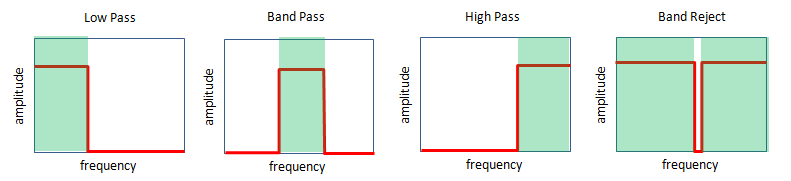
\includegraphics[scale=0.7]{{ImagesSSVEP/filter_types}.png}
    \caption{Τα τέσσερα βασικά είδη φίλτρων με βάση τις ζώνες συχνοτήτων που επιτρέπουν-απορρίπτουν. Αξίζει να σημειωθεί πως οι υποφαινόμενες αποκρίσεις στο πεδίο της συχνότητας, αναφέρονται σε ιδανικά φίλτρα (brick-wall filters), και πως στα πραγματικά, οι ζώνες αποκοπής δεν ορίζονται ποτέ από κάθετες γραμμές.}
    \label{fig:filter_types}
\end{figure}
\par Ένα άλλο κριτήριο με βάση το οποίο διαχωρίζονται τα φίλτρα είναι ο τρόπος με τον οποίο κάθε στιγμή χειρίζονται τις προηγούμενες εισόδους και εξόδους του συστήματος. Τα φίλτρα των οποίων η έξοδος εξαρτάται μόνο από τις προηγούμενες εισόδους ονομάζονται Φίλτρα Πεπερασμένης Κρουστικής Απόκρισης (Finite Impulse Response - FIR), ενώ αυτά που λαμβάνουν υπόψιν τους τόσο τις προηγούμενες εισόδους, αλλά και τις προηγούμενες εξόδους ονομάζονται Φίλτρα Άπειρης Κρουστικής Απόκρισης (Infinite Impulse Response - IIR). Το γεγονός πως τα IIR χρησιμοποιούν ένα είδος ανάδρασης (εξάρτηση από προηγούμενες εισόδους) είναι δυνατόν να τα καταστήσει ασταθή, πράγμα το οποίο δεν συμβαίνει με τα FIR, αν όμως χρησιμοποιηθεί με σωστό τρόπο, τότε, δεδομένων κάποιων συγκεκριμένων προδιαγραφών για ένα φίλτρο, μια IIR υλοποίηση θα ικανοποιήσει τις προδιαγραφές κάνοντας χρήση φίλτρου τάξης πολύ χαμηλότερης από το αντίστοιχο FIR, το οποίο μεταφράζεται σε λιγότερες πράξεις, άρα και σε λιγότερο υπολογιστικό χρόνο. 

\par Ένα από τα πιο κλασσικά IIR φίλτρα σχεδιάστηκε το 1930 απο το βρετανό μηχανικό και φυσικό Stephen Butterworth \cite{}. Βασικός στόχος του φίλτρου αυτού ήταν η επίτευξη σταθερής απόκρισης στη περιοχή διέλευσης συχνοτήτων, σε αντίθεση με τα μέχρι τότε φίλτρα τα οποία εμφάνιζαν διακυμάνσεις στην απόκρισή τους (ripple). Το τίμημα όμως για αυτήν την συμπεριφορά, είναι πως υπάρχει σχετικά μεγάλη απόκλιση στην περιοχή της συχνότητας αποκοπής, συγκριτικά με την απόκριση του αντίστοιχου ιδανικού φίλτρου.
\begin{figure}[H]
    \centering     %%% not \center
    \noindent\makebox[\textwidth]{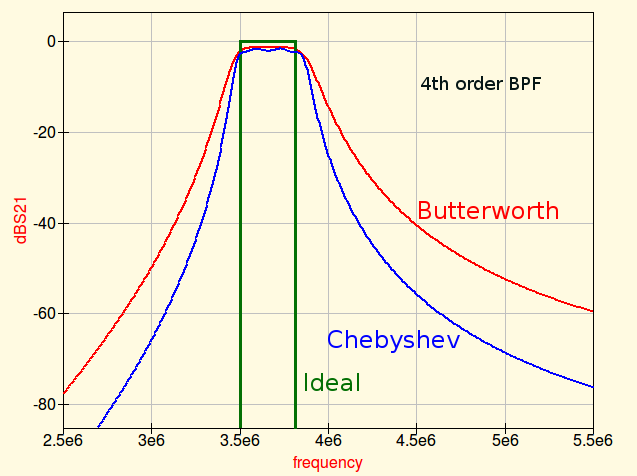
\includegraphics[scale=0.6]{{ImagesSSVEP/butter_cheby}.png}}
    \caption{Οι τρείς διαφορετικές αποκρίσεις για δύο διαφορετικά φίλτρα 3ης τάξης και του αντίστοιχου ιδανικού. Φαίνεται ξεκάθαρα η διακύμανση (ripple) στην ζώνη διέλευσης για ένα φίλτρο τύπου Chebyshev, η οποία δεν υπάρχει στο Butterwoth, καθώς και η μεγάλη απόκλιση του Butterworth σε σχέση με το ιδανικό, όσον αφορά τις δύο ζώνες αποκοπής. }
    \label{fig:butter_cheby}
\end{figure}
% add butte2
\section{Εξαγωγή χαρακτηριστικών}
\subsection{Canonical Correlation Analysis - CCA}

\par Η CCA είναι μια στατιστική μέθοδος που χρησιμοποιείται για την ανάλυση δομών δεδομένων, και συγκεκριμένα για την ανίχνευση της ομοιότητας μεταξύ δύο συνόλων μεταβλητών. Αυτό επιτυγχάνεται μέσω της εύρεσης δύο νέων συνόλων μεταβλητών, όπου το καθένα είναι γραμμικός συνδυασμός ενός από τα αρχικά σύνολα, έτσι ώστε να μεγιστοποιείται ο συντελεστής συσχέτισης τους. Κάνοντας χρήση μαθηματικού φορμαλισμού, έστω  
\section{Μηχανική Μάθηση}

\subsection{Principal Component Analysis - PCA}
\par Η Ανάλυση Κυρίων Συνιστωσών είναι μια στατιστική μέθοδος, που στο τομέα της μηχανικής μάθησης χρησιμοποιείται πολύ συχνά για την ελάττωση των χαρακτηριστικών (features) των δειγμάτων ενός συνόλου, επιλέγοντας μόνο εκείνα τα χαρακτηριστικά τα οποία συνεισφέρουν στην διατήρηση του μεγαλύτερου ποσοστού της μεταβλητότητας (variance) του συνόλου. Μια γεωμετρική ερμηνεία της παραπάνω διαδικασίας, είναι η προσπάθεια εύρεσης των κατευθύνσεων - αξόνων μέγιστης μεταβλητότητας των δεδομένων, και η προβολή τους σε κάποιους από αυτούς τους άξονες.
%ΕΙΚΟΝΑ 4 sub figures

\par Η χρησιμότητα της μεθόδου αυτής είναι εμφανής όταν έχουμε πολυδιάστατα δείγματα, όπως για παράδειγμα εικόνες  μεγέθους 16x16, δηλαδή δυανύσματα χαρακτηριστικών που ανήκουν στο $R^{256}$. Η χρήση όλων αυτών των χαρακτηριστικών σε έναν ακριβά υπολογιστικό αλγόριθμο μηχανικής μάθησης, όπως ο k-NN, θα επιβάρυνε σημαντικά την διαδικασία απόφασης, τόσο υπολογιστικά όσο και χρονικά. Με την χρήση της PCA όμως, είναι δυνατό να επιλεχθεί ένας αριθμός χαρακτηριστικών (π.χ 50-60), τα οποία να διατηρούν την πιο σημαντική στατιστική πληροφορία του συνόλου των εικόνων, με αποτέλεσμα να ελαττώνονται σημαντικά οι πόροι που χρείαζονται για την ταξινόμηση τους, χωρίς την εισαγωγή σημαντικού σφάλματος ταξινόμησης. Τέλος, ένα επιπλέον πλεονέκτημα, είναι πως σε πολλές περιπτώσεις, η PCA, βοηθάει στην αποφυγή του overfitting.

\par Όσον αφορά τον τρόπο υπολογισμού των κύριων συνιστωσών, θα δώσουμε ένα παράδειγμα, για ένα σύνολο δειγμάτων $X$ όπου το καθένα έχει δύο χαρακτηριστικά, δηλαδή $X_i \epsilon R^2$, όπου ο σκοπός μας είναι να του ελαττώσουμε την διάσταση κατά ένα. Αρχικά υπολογίζουμε τον πίνακα 
\begin{align}
\Sigma = \frac{1}{m}\sum_{i=1}^{i=m} X_i(X_i)^T \label{eq1}
\end{align}

\par Υποθέτοντας πως τα δεδομένα μας είναι κανονικοποιημένα έτσι ώστε $E[X_i]=0$ τότε η \eqref{eq1} ορίζει τον πίνακα συνδιασποράς του συνόλου $X$. Αποδεικνύεται πως η κατεύθυνση μέγιστης μεταβλητότητας $u_1$ (βλεπε εικόνα) αντιστοιχεί στο ιδιοδιάνυσμα που προκύπτει από την μεγαλύτερη ιδιοτιμή του πίνακα $\Sigma$. Αντίστοιχα η αμέσως επόμενη κατεύθυνση μέγιστης μεταβλητότητας $u_2$, αντιστοιχεί στο ιδιοδιάνυσμα που προκύπτει από την αμέσως μικρότερη ιδιοτιμή. Γενικεύοντας τώρα την παραπάνω πρόταση, αν τα δεδομένα μας $X_i \epsilon R^n$, και θέλουμε να τα προβάλουμε σε έναν υποχώρο διάστασης $R^k$, $k<n$, τότε πρέπει να διαλέξουμε τα $u_1,...,u_k$ να είναι τα ιδιοδιανύσματα που προκύπτουν από τις $k$ μεγαλύτερες ιδιοτιμές του πίνακα $\Sigma$, ο οποίος επειδή είναι συμμετρικός, τότε τα $u_i$, μπορούν πάντα να επιλέγονται έτσι ώστε να σχηματίζουν μια νέα ορθογώνια βάση για τα δεδομένα.

\par Στην συνέχεια του παραδείγματος μας τώρα, αφού υπολογίσουμε τα δύο ιδιοδιανύσματα $u_1$ και $u_2$ τότε μπορούμε να αναπαραστήσουμε τον πίνακα δεδομένων $X$, ως προς την ορθογώνια βάση $(u_1,u_2)$
\begin{align}
X_{rot} = U^TX =\begin{bmatrix}u_1^T\\u_2^T\end{bmatrix}X= \begin{bmatrix}u_1^TX\\u_2^TX\end{bmatrix}
\label{eq2}
\end{align}
\end{document}
 % Computational Methods Background Theory

\lhead{\emph{Κεφάλαιο 4}}

% !TEX root = ../Thesis.tex
% !TEX output_directory
\documentclass[11pt,a4paper,english,greek,twoside]{../Thesis}
\begin{document}
\chapter{Υλοποίηση SSVEP διεπαφής} \label{chap:SSVEP_implementation}
Στο κεφάλαιο 2, έγινε μια γενική περιγραφή των SSVEP σημάτων, και πως μπορούμε να τα χρησιμοποιήσουμε για την υλοποίηση διεπαφών μεταξύ εγκεφάλου και υπολογιστή. Σε αυτή την ενότητα θα γίνει παρουσίαση και αναλυτική περιγραφή της SSVEP διεπαφής που υλοποιήθηκε στα πλαίσια αυτής της διπλωματικής εργασίας \textcolor{red}{ΤΙΑΛΛΟ??}

\section{Υλικό}
%%%%%%%%%%%%%%%%%%%%%%%% General
\subsection{Εγκεφαλογράφος Emotiv Epoc}
\subsubsection{Περιγραφή}
\par Το σύστημα  Epoc από την εταιρεία Emotiv Systems, δημιουργήθηκε το 2009 και είναι ένας χαμηλού κόστους φορητός ασύρματος εγκεφαλογράφος, ο οποίος προοριζεται για χρήση σε παιχνίδια (gaming EEG system) και απλές εφαρμογές και όχι για να αντικαταστήσει τους κατα πολύ ακριβότερους εγκεφαλογράφους που χρησιμοποιούνται σε ιατρικές εφαρμογές . Το EPOC είναι μια πολύ συμπαγής κατασκευή, καθώς τα ηλεκτρόδια, ο ενισχυτής, τα κυκλώματα επεξέργασίας σήματος (DSP chips) αλλά και το σύστημα επικοινωνίας Bluetooth, είναι όλα ενσωματομένα σε μια πλακέτα μέσα στο EPOC , καθιστώντας το πολύ εύκολο στην μεταφορά και την χρήση. 
%Εικονα απο το εμοτιβ. 
\par Προσφέρει καταγραφή απο 16 ηλεκτρόδια τοποθετημένα σε πλαστικούς βραχίονες, και  καλύπτουν μια σχετικά ευρεία περιοχή του εγκεφάλου. Πιο συγκεκριμένα οι θέσεις που καλύπτουν τα ηλεκτρόδια, σύμφωνα με το διεθνές σύστημα 10-20 είναι οι : AF3, F7, F3, FC5, T7, P7, O1, O2, P8, T8, FC6, F4, F8, FC4, P3, και P4. Ο αισθητήρας στην θέση P3 (CMS) χρησιμοποιείται ώς ηλεκτρόδιο αναφοράς (reference), ενώ ο P4 (DRL) δρα ως feed-forward αντισταθμιστής των εξωτερικών αλλαγών που επηρεάζουν το συνολικό δυναμικό του σώματος, όπως οι παρεμβολές των 50Hz της τροφοδοσίας, οι μετασχηματιστές κ.α. 
%Eikona 10-20 me tous aisthitires
\par Επιπλέον, ενσωματομένα μέσα στον εγκεφαλογράφο βρίσκονται τόσο αναλογικά όσο και ψηφιακά φίλτρα. Αρχικά το σήμα κάθε αισθητήρα φιλτράρεται απο ένα υψιπερατό C-R φίλτρο με συχνότητα αποκοπής στα 0.16Hz, έπειτα περνάει απο ένα στάδιο προενίσχυσης και στην συνέχεια απο ένα βαθυπερατό φίλτρο με συχνότητα αποκοπής 83Hz. Στο επόμενο στάδιο γίνεται δειγματολειψία του σήματος από έναν αναλογικό σε ψηφιακό μετατροπέα (ADC) με συχνότητα δειγματοληψίας 2048Hz και το σήμα φιλτράρεται από ένα ψηφιακό sinc φίλτρο 5ης τάξης για την αφαίρεση της σύνηστώσας των 50Hz της τροφοδοσίας, και τέλος γίνεται υποδειγματοληψία στα 128Hz. Αν και ο ρυθμος αυτός (128Hz) είναι ικανός για την καταγραφή της σημαντικής εγκεφαλικής λειτουργίας, παραμένει σημαντικά μικρότερος απο τον ανίστοιχο ρυθμό άλλων εγκεφαλογράφων που προορίζονται για ιατρικές και ερευνητικές εφαρμογές (1000 – 2000Hz)

\subsubsection{Ηλεκτρόδια}
\par Τα ηλεκτρόδια με τα οποία είναι εξοπλισμένος ο EPOC, είναι ‘υγρού’ τύπου, παρόλαυτα διαφέρουν αρκετά ως προς την δομή συγκριτικά με τα ευρέως χρησιμοποιούμενα Ag/Ag-Cl που αναφέρθηκαν στην παράγραφο 1.2
Τα συγκεκριμένα, αποτελούνται απο ένα κυκλικό κομμάτι από ανοξείδωτο ατσάλι, επικαλυμένο απο μια λεπτή στρώση χρυσού. Η τελευταία στρώση αποτελείται από ένα πολυμερές υλικό υποδοχέα (polymer host) σε συνδυασμό με ένα ηλεκτρολυτικό, μη πολικό υλικό για το οποίο η εταιρεία δεν δίνει παραπανω πληροφορίες. Η επαφή με το δέρμα γίνεται μέσω μιας κυλινδρικής τσόχας πολυεστέρα (felt pad), την οποία σε κάθε χρήση, διαποτίζουμε σε αλατούχο διάλυμα (saline) για την ελλάτωση της αντίστασης επαφής.
εικονα
\par Το βασικό πρόβλημα από το οποίο υποφέρουν τα ηλεκτρόδια αυτά είναι η οξείδωση.  Παρα την λεπτή στρώση χρυσού που θα έπρεπε να την αποτρέπει, φαίνεται πως ένα απο τα άλλα υλικά της επίστρωσης, αντριδρά με το αλατούχο διάλυμμα και την προκαλεί. Σύμφωνα με το τεχνικό επιτελείο της εταιρείας, δεν έχει γίνει χημική ανάλυση για να διαπιστωθεί ακριβώς η αιτία της. Τέλος, επειδή παρατηρήθηκε πως η οξείδωση ξεκινάει πάντα απο την περιφέρεια του ηλεκτροδίου, είναι πολύ πιθανόν να μη είναι επαρκής η χρυσή επίστρωση σε αυτό το σημείο και να εκτίθεται το ανοξείδωτο ατσάλι στο αλατούχο διάλυμα, το οποίο αν είναι χαμηλής ποιότητας μπορεί να προκαλέσει την οξείδωση.
\par Η σημαντική επίπτωση που έχει η οξείδωση των ηλεκτροδίων δεν αφορά τόσο την ποιότητα του σήματος, καθώς δεν επηρεάζεται η αγωγιμότητα του ηλεκτροδίου, όσο την μηχανική δομή και αντοχή του ηλεκτροδίου. Παρατηρήθηκε πως μετά από το χρονικό διάστημα λίγων μηνών ξεκίνησε η θφορά στο πλαστικό σπέιρωμα του πλαστικού στηρίγματος του ηλεκτροδίου, ενώ σε παλιότερα ηλεκτρόδια που υπήρχαν στο εργαστήριο, το πλαστικό στήριγμα είχε σπάσει καθιστώντας το ηλεκτρόδιο εντελώς άχρηστο.
Εικονες απο σαπια ηλεκτρόδια
\par \textcolor{red}{(Συμβουλες για χρηση και διατηρηση ηλεκτροδίων ? )}

\subsubsection{Λογισμικό}
\textbf{Emotiv Sofware}
\par Μαζί με τον εγκεφαλογράφο Epoc, η Emotiv παρέχει μια σουίτα λογισμικού που προσφέρει στον χρήστη μια πληθώρα υπηρεσιών, άλλες δωρεάν και άλλες επί πληρωμή. 
Η βασική και δωρεάν εφαρμογή, είναι η EMOTIV Xavier Control Panel, η οποία βοηθάει τον χρήστη να κάνει την εγκατάσταση του Epoc, και να μάθει να το χρησιμοποιεί Δίνεται η δυνατότητα στον χρήστη να παρακολουθεί την ποιότητα επαφής των ηλεκτροδίων με το δέρμα αναπαριστώντας με πράσινο χρώμα την καλή ποιότητα, τις ενδιάμεσες καταστάσεις με κίτρινο και κόκκινο, ενώ μαύρο χρησιμοποιείται όταν πρακτικά λαμβάνεται μόνο θόρυβος.
%Εικονα
\par Μια άλλη λειτουργία που παρέχεται, είναι ο υπολογισμός πέντε μετρικών εγκεφαλικής λειτουργίας σε πραγματικό χρόνο : engagement, συγκέντρωση, ενδιαφέρων, χαλάρωση, άγχος.
%Εικονα
\par Τέλος παρέχεται ένα σύστημα το οποίο είναι ικανό να εκπαιδευθεί από τον κάθε χρήστη ξεχωριστά, έτσι ώστε να ξεχωρίζει συγκεκριμένες σκέψεις και να τις αντιστοιχίζει σε ξεχωριστές λειτουργίες που θα επιλέξει ο χρήστης, όπως η μετακίνηση και περιστροφή ενός εικονικού αντικειμένου ή ο έλεγχος του δείκτη του ποντικιού. Η επιτυχία αυτού του συστήματος εξαρτάται σε μεγάλο βαθμό από τον χρόνο που θα επενδύσει κάποιος στην εκπαίδευση του, καθώς και από την ικανότητα του να συγκεντρώνεται και να διαχωρίζει τις σκέψεις του. Ενδεικτικά μετά από ένα χρονικό διάστημα 10 λεπτών, κατάφερα να μετακινώ έναν εικονικό τρισδιάστατο κύβο μπροστά και πίσω κατά βούληση, παρόλαυτα όταν προσπάθησα να εισάγω παραπάνω εντολές (περιστροφή δεξιόστροφη και αριστερόστροφη), τότε ήταν σχεδόν αδύνατο να ελέγξω τον κύβο όπως πριν.
εικόνα

\textbf{Emokit}
\par Προκειμένου όμως ένας χρήστης να αποκτήσει πρόσβαση στις μετρήσεις κάθε αισθητήρα ξεχωριστά, δηλαδή στο εγκεφαλογράφημα αυτό καθ’ αυτό, θα πρέπει αγοράσει την ερευνητική έκδοση του EPOC (research Edition). Με αυτή την έκδοση, η Emotiv παρέχει το ερευνητικό κιτ αναπτυξης λογισμικού (research SDK) το οποίο μπορεί να χρησιμοποιειθεί με μια πληθώρα προγραμματιστικών γλωσσών (C++, Python, Matlab, Java, C\#) για την επεξεργασία των εγκεφαλικών σημάτων. Το γεγονός όμως πως ο εγκεφαλογράφος που υπήρχε στο εργαστήριο δεν ήταν η ερευνητική έκδοση, απαιτούσε την εύρεση λύσης σε ελέυθερο λογισμικό το οποίο να παρέχει δυνατότητες παρόμοιες με αυτές του research SDK απο την Emotiv. Μια τέτοια βιβλιοθήκη είναι η Emokit και δημιουργήθηκε από την ομάδα προγραμματιστών στην OpenYou, και δίνει πρόσβαση στις μετρήσεις των αισθητήρων, την ποιότητα της επαφής και την στάθμη της μπαταρίας της συσκευής. Επιπλέον, δίνεται η δυνατότητα εξαγωγής των αποτελεσμάτων σε μορφή csv, καθώς και η αντίστροφη διαδικασία, κατά την οποία ένα csv αρχείο “διαβάζεται” σε πραγματικό χρόνο, παίζοντας τον ρόλο του εγκεφαλογράφου.

\par Στην βιβλιοθήκη συμπεριλαμβάνονται και κάποια script που υποδυκνείουν τους βασικούς τρόπους χρήσης. Αρχικά τρέχοντας το example.py εμφανίζεται ένας πίνακας με την τιμή, και την ποιότητα για κάθε ηλεκτρόδιο, τις τιμές για τον γυροσκοπικό αισθητήρα καθώς και την στάθμη της μπαταρίας.
ΕΙΚΟΝΑ 
\par Αυτού του είδους η απεικόνιση είναι μάλλον άβολη για μελέτη των εγκεφαλικών σημάτων και πιο πολύ χρησιμεύει ως ένας γρήγορος έλεγχος της ποιότητας σύνδεσης του EPOC με τον υπολογιστή.
Ένας πολύ διαφορετικό τρόπος απεικόνισης υλοποιείται στο αρχείο render.py όπου κάνοντας χρήση της βιβλιοθήκης pygame απεικονίζονται σε πραγματικό χρόνο τα διαγράμματα τιμών για κάθε ηλεκτρόδιο ξεχωριστά. Επίσης το χρώμα της γραφικής παράστασης εξαρτάται από την ποιότητα της επαφής του ηλεκτροδίου με το δέρμα. Το γραφικό περιβάλλον φαίνεται στην εικόνα (). 
ΕΙΚΟΝΑ
\par Παρότι αυτού του είδους η απεικόνιση είναι πολύ χρήσιμη, ένα βασικό προβλημα που φαίνεται και στην ΕΙΚΟΝΑ, είναι πως τα σήματα που δίνει το EPOC περιέχουν offset, με αποτέλεσμα πολλές φορές οι γραφικές παραστάσεις μπέρδευονται μεταξύ τους. Επίσης δεν παρέχεται καθόλου συχνοτική πληροφορία για κάθε κανάλι, πράγμα το οποίο θα βοηθούσε στην γρήρορη οπτικοποίηση των SSVEP σημάτων.
\par Κρίθηκε σημαντικό λοιπόν, στα πλαίσια της παρούσας διπλωματικής εργασίας, να αναπτυχθεί μια γραφική διεπαφή για την οπτικοποίηση των εγκεφαλικών σημάτων, σε Python 2.7,  με τα εξής χαρακτηριστικά :
\begin{itemize}
    \item{Χρήση του εργαλείου pyqtgraph για την δημιουργία του γραφικού περιβάλλοντος}
    \item{Ενσωμάτωση φίλτρων για την αφαίρεση του offset, και λοιπών συχνοτήτων που μπορεί να μην ενδιαφέρουν.}
    \item{Εμφάνιση του διαγράμματος Power Spectrum Density για κάθε κανάλι,  με δυνατότητα επιλογής του παραθύρου υπολογισμού του μετασχηματισμού Fourier}
    \item{Τα χρώματα των γραφικών παραστάσεων να βασίζονται στην τιμή ποιότητας για κάθε κανάλι.}
    \item{Ενδείξεις για την ακριβή τιμή της ποιότητας καθώς και για το συχνοτικό peak, στο γράφημα του χρόνου και της συχνότητας αντίστοιχα.}
\end{itemize}

ΕΙΚΟΝΑ-ΕΙΚΟΝΕΣ

\subsection{Υπολογιστής}
\par Η όλη εφαρμογή υλοποιήθηκε σε έναν φορητό υπολογιστή ASUS με επεξεργαστή Intel Pentium i7 και χρησιμοποιώντας το λειτουργικό σύστημα Ubuntu. Παρότι η βιβλιοθήκη Emokit υποστηρίζεται τόσο για Windows όσο και για Unix λειτουργικά, διάφορα προβλήματα που παρουσιάστηκαν στην επικοινωνία του EPOC με τον υπολογιστή στο Windows περιβάλλον, ώθησαν στην επιλογή του Ubuntu.

\subsection{Συστοιχίες LED}
\par Στην υποενότητα \ref{subsec:visual_stimulus} αναλύθηκαν οι πιο συχνοί τρόποι που χρησιμοποιούνται για την επίτευξη της επαναλαμβανόμενης οπτικής διέγερσης (ΕΟΔ), τα πλεονεκτήματα και μειονεκτήματα της κάθε μιας καθώς και τους λόγους που στην παρούσα εργασία επιλέχθηκαν τα LED. Σε αυτήν την ενότητα θα γίνει μια παρουσίαση των LED συστοιχιών που κατασκευάστηκαν καθώς και της βάσης τους η οποία προσαρμόζεται στην οθόνη ενός φορητού υπολογιστή.

\subsubsection{Επιλογή χρώματος LED}
\par Ένας από τα βασικά χαρακτηριστικά των LED, που παίζει σημαντικό ρόλο στην ποιότητα των SSVEP σημάτων που θα προκληθούν στον εγκέφαλο, είναι το χρώμα των LED. 
ΧΧΧ
ΠΕΣ ΓΙΑ ΈΡΕΥΝΕΣ, ΓΙΑ 3 ΚΑΜΠΎΛΕΣ ΣΤΟ ΜΆΤΙ (RGB), 
Παρότι τα άσπρου χρώματος LED φαίνεται να αποδίδουν καλύτερα, σε δοκιμές που κάναμε χρησιμοποιώντας μια συστοιχία 25 LEDs, διατεταγμένα 5x5,  παρατηρήθηκε πολύ έντονη κόπωση των ματιών σε όλα τα άτομα που δοκίμασαν να κοιτάξουν τα LED. Συγκεκριμένα, ήταν αδύνατο να κρατήσουν οπτική επαφή για πάνω από 1 λεπτό, συνεπώς ενώ τα άσπρα LED παρήγαγαν πολύ δυνατά SSVEP σήματα σε όλα τα άτομα, έπρεπε να επιλεχθούν LED διαφορετικού χρώματος.
ΕΙΚΟΝΑ ΑΠΟ SSVEP WHITE LEDS
Έπειτα από δοκιμές με κόκκινα και πράσινα LED, παρατηρήθηκε πολύ μικρή διαφορά στα παραγόμενα SSVEP σήματα, συνεπώς καταλήξαμε στα πράσινα όντας τα πιο ξεκούραστα για το μάτι, ακόμα και σε πολύ δυνατές φωτεινές εντάσεις.

\subsubsection{Σχηματικό και Κατασκευή}
\par Στην συγκεκριμένη διεπαφή θα χρησιμοποιήσουμε 4 πηγές φωτός οπού η κάθε μία θα αναβοσβήνει με διαφορετική συχνότητα, συνεπώς θα χρειαστούν 4 συστοιχίες LED. Ο αριθμός των LED για κάθε συστοιχία επιλέχθηκε να είναι 20, σε διάταξη 5x4. Επιλέχθηκε μεγάλος αριθμός έτσι ώστε επηρεάζοντας την τροφοδοσία των led, να υπάρχει δυνατότητα πειραματισμού με την ένταση του φωτισμού, η οποία μπορεί να κυμαίνεται από αμυδρό φωτισμό των led, μέχρι πολύ δυνατή ένταση που κουράζει γρήγορα τα μάτια. Επιπλέον, σε κάθε συστοιχία προστέθηκε ένα επιπρόσθετο κόκκινο LED διαμέτρου 3mm, του οποίου η χρησιμότητα είναι διττή. Κατά την διάρκεια της offline ανάλυσης των σημάτων θα σηματοδοτεί ποια συστοιχία θα πρέπει να κοιτάξει το εκάστοτε άτομο, ενώ κατά την διάρκεια της online χρήσης της διεπαφής, θα επισημαίνει την συστοιχία στην οποία ανιχνεύεται ότι έχει στραμμένο το βλέμμα του. Κάθε συστοιχία υλοποιήθηκε πάνω σε ένα stripboard όπου καθένα από αυτά θα ενσωματωνεται σε μια ξύλινη βάση που μπορεί να προσαρμόζεται σε κάθε είδους λεπτή οθόνη. Στην εικόνα ΧΧΧ φαίνεται το κυκλωματικό διάγραμμα, ο φυσικός σχεδιασμός του στο stripboard, καθώς και η τελειωμένη κατασκευή.

\par EIKONESr 
\par Τα LED που επιλέχθηκαν έπρεπε να ικανοποιούν δύο βασικές προυποθέσεις: 
\begin{itemize}
    \item{Nα έχουν πολύ καλή απόδοση.}
    \item{Nα έχουν ευρεία γωνία θέασης.}
\end{itemize} 
\par Τα LED που επιλέχθηκαν είναι  τα ΤΑΔΕ με γωνια θεασης ΤΑΔΕ και 

\subsubsection{Κύκλωμα Οδήγησης}
\par Για τις απαιτήσεις του πειράματος απαιτούνταν ο πλήρης έλεγχος των LED, δηλαδή η δυνατότητα ξεχωριστών σημάτων ελέγχου για κάθε μια από τις 4 συστοιχίες, καθώς και για τα 4 κόκκινα LEDs συνεπώς χρειάζεται ένας μικρο-ελεγκτής με τουλάχιστον 8 ψηφιακές εξόδους, καθώς και να είναι πολύ μικρός σε μέγεθος έτσι ώστε να ενσωματωθεί εύκολα στην συνολική πλακέτα οδήγησης. Τελικώς, χρησιμοποιήθηκε ο μικροελεγκτής Arduino Nano, που παρέχει 22 ψηφιακές θύρες εισόδου/εξόδου καθώς και ειδικούς ακροδέκτες που καθιστούν εύκολη την εφαρμογή του σε πλακέτες.  
\par Κάθε συστοιχία αποτελείται από 20 LEDs και κάθε LED χρειάζεται περίπου 3mA για να παράγει επαρκή φωτεινότητα για τις απαιτήσεις του πειράματος, συνεπώς το ρεύμα που απαιτείται για την οδήγηση κάθε συστοιχίας είναι περίπου 60mA, το οποίο ξεπερνάει το μέγιστο ρέυμα που μπορει να διαχειριστεί κάθε εξοδος του Arduino (40mA). Συνεπώς θα χρησιμοποιήθούν 8 τρανζίστορ, ένα για κάθε συστοιχία και ένα για κάθε κόκκινο LED. Το κύκλωμα μπορεί να τροφοδότηθεί είτε από την θύρα Vin του arduino, που ταυτίζεται  με την  έξοδο των 5volt της θύρας USB στην οποία συνδέεται, είτε από εξωτερική DC τροφοδοσία, καθώς στο κύκλωμα περιλαμβανεται o σταθεροποιητής τάσης LM317. Στην εικόνα ΧΧΧ φαίνεται το κυκλωματικό διάγραμμα, ο φυσικός σχεδιασμός του στο stripboard, καθώς και η τελειωμένη κατασκευή.
%mhpws na mhn prodidw to caption ap thn paragrafo
\par ΕΙΚΟΝΑ  
 
\subsubsection{Λογισμικό Arduino}
\par Όπως έχει αναφερθεί, ο σκοπός που πρέπει να επιτευχθεί είναι κάθε συστοιχία να αναβοσβήνει με την δικής της συχνότητα ανεξάρτητα από τις άλλες. Είναι σημαντικό να υπάρχει απόλυτη ακρίβεια στην συχνότητα, και ευκολία στην επιλογή της κάθε μίας, για να διευκολυνθεί η διαδικασία των πειραματισμών. Προς την ίδια κατεύθυνση θέλουμε να υπάρχει και η δυνατότητα επιλογής διαφορετικού duty cycle για κάθε συστοιχία καθώς,  όπως θα φανεί και στην συνέχεια, επηρεάζει την ποιότητα των SSVEP σημάτων. Ενώ είναι πολύ εύκολο να επιτευχθεί η δημιουργία τετραγωνικού παλμού σε μια ψηφιακή έξοδο του Arduino, πχ ρυθμίζοντας ακριβώς τον χρόνο που θα είναι On και Off με την χρήση της εντολής delay(), η επέκταση αυτής της λειτουργίας και σε άλλες εξόδους ταυτόχρονα απαιτεί την χρήση την χρήση ενώς thread για κάθε διαφορετική έξοδο, τα οποία να εργάζονται παράλληλα. Για αυτό το λόγο χρησιμοποιήθηκε η βιβλιοθήκη Timer του Simon Monk η οποία επιτελεί αυτόν ακριβώς τον σκοπό. Παρόλαυτά δεν παρέχεται η δυνατότητα επιλογής duty cycle, το οποίο παραμένει σταθερά στο $50\%$. Για τον λόγο αυτό τροποποιήθηκε o πυρήνας της βιβλιοθήκης ετσι ώστε ο χρήστης να μπορεί να θέσει ακριβώς την διάρκεια On και Off του παλμού.  Στην εικόνα \#ΕΙΚΟΝΑ φαίνεται η δημιουργία παλμού με την χρήση της delay(), της βιβλιοθήκης Timer.
\par EIKONA

\par Τέλος, επειδή η κατάσταση  των LED πρέπει να ελέγχεται πλήρως από την διεπαφή, η οποία θα είναι γραμμένη σε  Python, χρησιμοποιήθηκε η βιβλιοθήκη Pyserial, έτσι ώστε η διεπαφή και το Arduino να επικοινωνούν σειριακά μέσω της USB θύρας. Με αυτό τον τρόπο είναι δυνατός ο έλεγχος της εκκίνησης η της παύσης των LEDs, καθώς και των κόκκινων ενδεικτικών LEDs.

\begin{table}
	\centering
    \begin{tabular}{| l | l | l | l |}
    \hline
    \textbf{Metric} & \textbf{Value} \\ \hline
    Accuracy & 77.95\% \\ \hline
    Recall & 0.91 \\ \hline
    Precision & 0.87 \\ \hline
    F1-score & 0.88 \\
    \hline
    \end{tabular}
	\caption{Αποτελέσματα 4 μετρικών για την ανίχνευση αντικειμένων πάνω σε όλα τα βίντεο του συνόλου δεδομένων test που χρησιμοποιήσαμε. Παρατηρούμε ότι με σύζευξη λόγου και εικόνας μπορούμε να πετύχουμε ικανοποιητικά αποτελέσματα, πολύ πιο εύρωστα από ό,τι με χρήση μόνο ενός από τους δύο τρόπους.}
	\label{tab:ObjeResult}
\end{table}

\cite{lawrence_waves}
\end{document}
 % SSVEP implementation

%% ----------------------------------------------------------------
% Now begin the Appendices, including them as separate files
%%\addtocontents{toc}{\vspace{2em},\protect\setcounter{tocdepth}{-1}}
%\addtocontents{toc}{\vspace{2em}} % Add a gap in the Contents, for aesthetics
% \begin{appendices} % Cue to tell LaTeX that the following 'chapters' are Appendices
% % !TEX root = ../Thesis.tex
% !TEX output_directory = ../
\chapter{Το Σύνολο Δεδομένων Και Οι Τροποποιήσεις Στις Οποίες Προβήκαμε} \label{dataset}




\begin{table}
	\begin{tabular}{|p{13.5cm}|}
		\hline
		Actions in MPII Cooking Activities Dataset \\ \hline
		Background activity, change temperature, cut apart, cut dice, cut in, cut off ends, cut out inside, cut slices, cut stripes, dry, fill water from tap, grate, lid: put on, lid: remove, mix, move from X to Y, open egg, open tin, open/close cupboard, open/close drawer, open/close fridge, open/close oven, package X, peel, plug in/out, pour, pull out, puree, put in bowl, put in pan/pot, put on bread/dough, put on cutting-board, put on plate, read, remove from package, rip open, scratch off, screw close, screw open, shake, smell, spice, spread, squeeze, stamp, stir, strew, take \& put in cupboard, take \& put in drawer, take \& put in fridge, take \& put in oven, take \& put in spice holder, take ingredient apart, take out from cupboard, take out from drawer, take out from fridge, take out from oven, take out from spice holder, taste, throw in garbage, unroll dough, wash hands, wash objects, whisk, wipe clean. \\
		\hline
	\end{tabular}
	\caption{Οι 65 δράσεις του συνόλου δεδομένων MPII Cooking Activities Dataset. Στα πειράματά μας, οι δράσεις put on cutting-board, read και smell ενσωματώνονται στην κατηγορία background activity και η δράση wash hands συνενώνεται με τη δράση wash hands.}
	\label{tab:DataActions}
\end{table}



\par Τα 44 βίντεο ακολουθούν μια σύμβαση ονομασίας τύπου sSS-dDD, με τα SS και DD να αποτελούν διψήφιους αριθμούς που υποδεικνύουν το υποκείμενο, δράστη του βίντεο που εκτελεί τη συνταγή, (s από το subject) και το πιάτο-συνταγή (d από το dish) αντίστοιχα. Για παράδειγμα, έγκυρη ονομασία είναι η s19-d07, που υποδηλώνει ότι ο δράστης 19 εκτελεί τη συνταγή 7. Στο σύνολο των 44 βίντεο, εμφανίζονται διάφοροι συνδυασμοί υποκειμένων από το 8 ως το 20 και πιάτων από το 1 ως το 14. Είναι φανερό ότι το σύνολο δεδομένων περιέχει ένα υποσύνολο όλων των πιθανών συνδυασμών δραστών και συνταγών. Τα βίντεο που περιέχονται φαίνονται στον πίνακα \ref{tab:DataVideos}. Από αυτά, επιλέχθηκαν ως βίντεο εκπαίδευσης όσα αφορούν τους δράστες 11 ως 15. Επειδή κάποιες κατηγορίες δεν περιέχονταν στα βίντεο αυτά, προσθέσαμε στα βίντεο εκπαίδευσης επιπλέον τα s08-d02 και s10-d10. Όλα τα βίντεο είναι πυκνά δειγματοληπτημένα στα 29.4 frames ανά δευτερόλεπτο. Η συνολική διάρκεια των βίντεο, εκπαίδευσης και ελέγχου είναι περίπου 8 ώρες, επομένως ο αριθμός των συνολικών frames ξεπερνά τις 800000.

\begin{table}
    \begin{tabular}{|p{13.5cm}|}
    \hline
    Videos in MPII Cooking Activities Dataset \\ \hline
    s08-d02, s08-d04, s08-d11, s08-d14, s10-d02, s10-d10, s10-d11, s11-d01, s11-d06, s11-d11, s11-d12, s11-d13, s11-d14, s12-d05, s12-d07, s12-d09, s12-d10, s12-d14, s13-d08, s13-d09, s13-d11, s13-d12, s13-d13, s14-d08, s14-d09, s14-d11, s15-d03, s15-d07, s15-d14, s16-d01, s16-d06, s16-d09, s16-d11, s17-d02, s17-d05, s17-d13, s18-d11, s19-d01, s19-d06, s19-d07, s19-d09, s19-d10, s19-d12, s20-d07. \\
    \hline
    \end{tabular}
	\caption{Τα 44 βίντεο του συνόλου δεδομένων MPII Cooking Activities Dataset. Από αυτά, χρησιμοποιούμε για εκπαίδευση όσα αφορούν τους δράστες 11 ως 15 και τα s08-d02 και s10-d10.}
	\label{tab:DataVideos}
\end{table}



\par Το σύνολο MPII Cooking 2 Dataset περιέχει επισημειώσεις αρκετά πλουσιότερες αυτών του MPII Cooking Activities Dataset. Αρχικά, παρέχονται επισημειώσεις δράσεων για κάθε βίντεο στη μορφή: έναρξη (σε χρόνο και frames) και λήξη δράσης, είδος δράσης, δράστης και σύνολο αντικειμένων που πλαισιώνουν τη δράση. Τα αντικείμενα αυτά χωρίζονται επιπλέον σε εργαλεία και υλικά, αλλά η διάκριση αυτή δεν αφορά την εργασία μας. Με βάση τις επισημειώσεις αυτές, αποκτούμε έναν χρονικό χάρτη των αντικειμένων που εμφανίζονται στο βίντεο. Βέβαια υπογραμμίζουμε το ότι οι επισημειώσεις αυτές αφορούν τα αντικείμενα που χρησιμοποιούνται στην κάθε δράση και όχι αυτά που εμφανίζονται οπτικά στο βίντεο σε κάθε χρονική στιγμή. Τα αντικείμενα που εμφανίζονται κατατάσσονται σε 155 κατηγορίες, από τις οποίες μας ενδιαφέρουν μόνο οι 92, καθώς αυτές εμφανίζονται στα βίντεο του MPII Cooking Activities Dataset. Επιπλέον, στις 92 κατηγορίες δεν περιλαμβάνονται συγκεκριμένα ουσιαστικά όπως χέρι και πάγκος, καθώς δεν δίνουν ιδιαίτερη πληροφορία για τη δράση. Το σύνολο των ουσιαστικών που χρησιμοποιούνται στα πειράματά μας φαίνεται στον πίνακα \ref{tab:DataNouns}.

\begin{table}
    \begin{tabular}{|p{13.55cm}|}
    \hline
    Objects in MPII Cooking 2 Dataset \\ \hline
    apple, baking tray, blender, bottle, bowl, box grater, bread, bread knife, butter, carrot, cheese, chefs knife, chocolate, colander, corn, cucumber, cup, cupboard, dough, drawer, egg, eggshell, electricity column, electricity plug, flat grater, fridge, front peeler, frying pan, garbage, garlic clove, glass, ham, hot chocolate powder bag, jar, kiwi, knife, kohlrabi, ladle, lemon, lid, masher, measuring pitcher, milk, mushroom, oil, onion, orange, oven, paper, paper box, peach, pear, peel, pepper, pineapple, plastic bag, platic bottle, plastic box, plastic paper bag, plate, plum, pot, potato, puree, salad, salami, salt, seed, side peeler, sink, soup, spatula, spice, spice holder, spice shaker, sponge, sponge cloth, spoon, squeezer, stone, stove, tap, teaspoon, tin, tin opener, tomato, towel, water, wire whisk, wrapping paper, yolk, zucchini. \\
    \hline
    \end{tabular}
	\caption{Οι 92 κατηγορίες αντικειμένων που εμφανίζονται στα βίντεο του συνόλου MPII Cooking Activities Dataset και που χρησιμοποιούμε στα πειράματά μας.}
	\label{tab:DataNouns}
\end{table}


\section{Επιπλέον Επισημειώσεις Στις Οποίες Προβήκαμε}
\subsection{Υπότιτλοι}
Για την αξιοποίηση της ομιλίας ως τρόπο έκφρασης επιπλέον πληροφορίας, προβαίνουμε σε ανάλυση υποτίτλων, ώστε να αποφύγουμε τα σφάλματα που θα εισήγαγε ένα σύστημα αυτόματης αναγνώρισης λόγου, καθώς αυτό ξεφεύγει από τον σκοπό αυτής της εργασίας. Επειδή δεν υπάρχουν υπότιτλοι για το MPII Cooking Activities Dataset, δημιουργήσαμε εμείς. Σε ένα σύνολο επισημειωτών δόθηκε το βίντεο και οι επισημειώσεις δράσεων και αντικειμένων από το MPII Cooking 2 Dataset. Επιβάλλαμε τον περιορισμό της χρήσης των ονομάτων των αντικειμένων απευθείας και όχι συνωνύμων τους, καθώς στη χρήση των υποτίτλων αναζητούμε μόνο τα ονόματα των αντικειμένων όπως αυτά παρέχονται από το MPII Cooking 2 Dataset. Όσον αφορά τους χρόνους ενός επιλόγου, επιβάλλαμε να εκτείνονται εντός της διάρκειας της δράσης και το χρονικό τους μήκος να περιορίζεται κάτω από τα 15 δευτερόλεπτα, ανάλογα πάντα με το μέγεθος του διαλόγου σε λέξεις. Προσπαθήσαμε να διατηρήσουμε τη φυσικότητα των υποτίτλων και ταυτόχρονα να διευκολύνουμε την ανίχνευση αντικειμένων μέσω αυτών. Στον πίνακα \ref{tab:DataSubtitles} φαίνεται ένα παράδειγμα τμήματος των υποτίτλων για το βίντεο s08-d04.

\begin{table}
    \begin{tabular}{ | l | l | l |}
    \hline
    Start Time & End Time & Subtitle \\ \hline
    714.7200 & 722.7210 & Pour enough oil to fill the bottom of your frying-pan. \\ \hline
	723.0950 & 726.9380 & Spread it uniformly. \\ \hline
	728.4170 & 730.6840 & Ok, turn on the stove in this point. \\ \hline
	730.7240 & 734.8660 & Choose a high temperature for start. \\
    \hline
    \end{tabular}
	\caption{Παράδειγμα υποτίτλων για το βίντεο s08-d04. Όλοι οι χρόνοι αναφέρονται σε δευτερόλεπτα από την αρχή του βίντεο.}
	\label{tab:DataSubtitles}
\end{table}


\subsection{Επισημειώσεις Αντικειμένων}
Το σύνολο MPII Cooking 2 Dataset περιέχει επισημειώσεις για τα αντικείμενα που χρησιμοποιούνται ανά δράση. Ωστόσο, οπτική επισημείωση, για τη θέση δηλαδή του χρησιμοποιούμενου αντικειμένου στα frames, δεν υπάρχει. Προκειμένου να εντοπίσουμε οπτικά τα αντικείμενα στα frames του βίντεο, είναι φανερό ότι πρέπει να έχουμε δεδομένα για την εμφάνιση τους. Καθώς η μεταβλητότητα των αντικειμένων είναι εξαιρετικά μεγάλη (όπως αναλύουμε στο κεφάλαιο 4), δημιουργούμε μοντέλα αντικειμένων για κάθε βίντεο ξεχωριστά. Η δημιουργία επισημειώσεων έγινε σε δύο στάδια, τα οποία εξυπηρετούν διαφορετικούς σκοπούς.

\par Σε πρώτη φάση, δειγματοληπτούμε το βίντεο με περίοδο 100 frames και σε κάθε ένα σημειώνουμε τα αντικείμενα που εμφανίζονται. Η διαδικασία αυτή γίνεται με τη λειτουργία trainingImageLabeler του λογισμικού MATLAB. Με το λογισμικό αυτό, είναι εύκολο να δημιουργηθεί ένα ορθογώνιο που περιλαμβάνει την περιοχή ενδιαφέροντος. Ο χρήστης εισάγει τα ορθογώνια και τις ετικέτες και το πρόγραμμα εξάγει τις χωρικές συντεταγμένες πάνω στο frame. Ένα παράδειγμα φαίνεται στην παρακάτω εικόνα:

\begin{figure}[H]
  \centering
  \noindent\makebox[\textwidth]{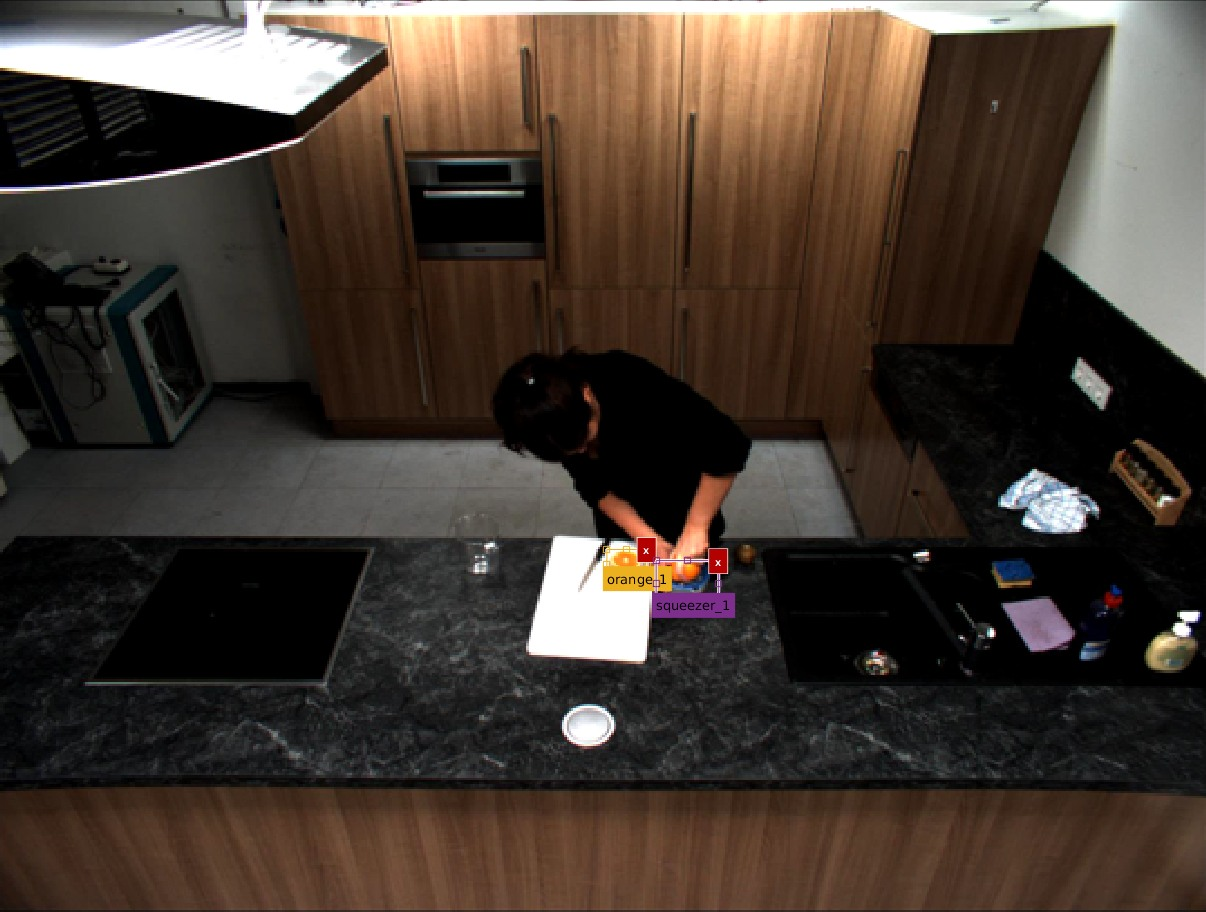
\includegraphics[scale=0.25]{{Images/AppMatlab}.jpg}}
  \caption{Παράδειγμα δημιουργίας επισημειώσεων με το λογισμικό trainingImageLabeler του MATLAB. Εισάγουμε τα ορθογώνια και την ετικέτα και το λογισμικό εξάγει τις συντεταγμένες. Η χρήση του πακέτου αυτου διευκολύνει τη μαζική δημιουργία θετικών δειγμάτων εκπαίδευσης για ανιχνευτές αντικειμένων.}
  \label{fig:AppMatlab}
\end{figure}



\begin{figure}[H]
  \centering
  \noindent\makebox[\textwidth]{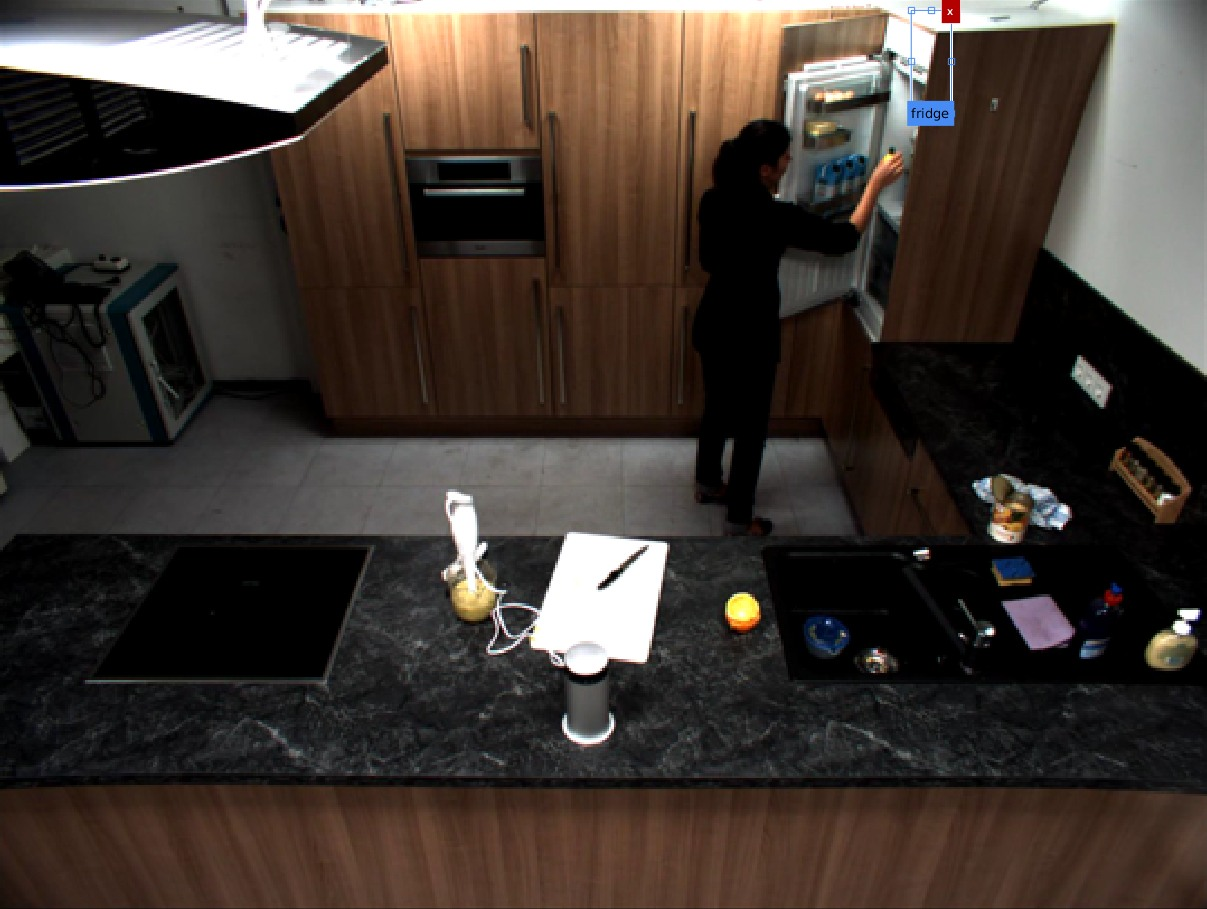
\includegraphics[scale=0.25]{{Images/AppFridge}.jpg}}
  \caption{Παράδειγμα αναπαράστασης σταθερού αντικειμένου με το τμήμα του το οποίο εμφανίζεται μόνο όταν το αντικείμενο χρησιμοποιείται. Έτσι, εξασφαλίζεται ότι το αντικείμενο θα εντοπίζεται μόνο σε περιπτώσεις ενδιαφέροντος και όχι σε όλη τη διάρκεια του βίντεο.}
  \label{fig:AppFridge}
\end{figure}

\par Οι επισημειώσεις αυτές λειτουργούν ως θετικά δείγματα για εκπαίδευση ενός ανιχνευτή αντικειμένων. Λόγω της υψηλής μεταβλητότητας, επιλέξαμε τη χρήση Ταιριάσματος Προτύπων (Template Matching) ως ανιχνευτή αντικειμένων κι έτσι απαιτούνταν να συλλέξουμε πρότυπα. Έχοντας λοιπόν τις πλήρεις επισημειώσεις μέσω του trainingImageLabeler, επιλέξαμε αυτές που εμφανίζοταν συχνά και για μεγάλη χρονική διάρκεια ως αντιπροσώπους κλάσεων αντικειμένων. Πρακτικά, συρρικνώνουμε τα θετικά δείγματα έτσι ώστε να ελαχιστοποιείται η απώλεια που αυτό συνεπάγεται στην μεταβλητότητα και στον ικανοποιητικό εντοπισμό. Στο κεφάλαιο 4 αναλύουμε περισσότερα για τη μέθοδο εντοπισμού των αντικειμένων.


\subsection{Επισημειώσεις Χεριών}
Στο κεφάλαιο 5 δείχνουμε τον εντοπισμό χεριών και την εξαγωγή του τύπου λαβής (grasping type). Στο κεφάλαιο 6, τα αποτελέσματα φαίνονται να υποβοηθούνται από αυτή την πληροφορία. Εν τούτοις, σύνολο δεδομένων δεν υπήρχε ούτε σχετικά με τον εντοπισμό χεριών, ούτε σχετικά με την εξαγωγή τύπου λαβής, που να σχετίζονται άμεσα με το MPII Cooking Activities Dataset. Επομένως, έπρεπε να δημιουργήσουμε, με βάση τις διαθέσιμες πληροφορίες, μια βάση για τον εντοπισμό χεριών αρχικά.


\par Η έλλειψη επισημειώσεων για τον τύπο λαβής μας ανάγκασε να χρησιμοποιήσουμε μη επιβλεπόμενη μάθησης, όπως περιγράφεται στο κεφάλαιο 5. Επομένως, δημιουργούμε ένα σύνολο δεδομένων τύπων λαβής με αυτόματο τρόπο, λύνοντας το πρόβλημα απουσίας επισημειώσεων και δεν προβαίνουμε σε επιπλέον διαδικασίες επισημειώσεων.

\begin{figure}
  \centering
  \noindent\makebox[\textwidth]{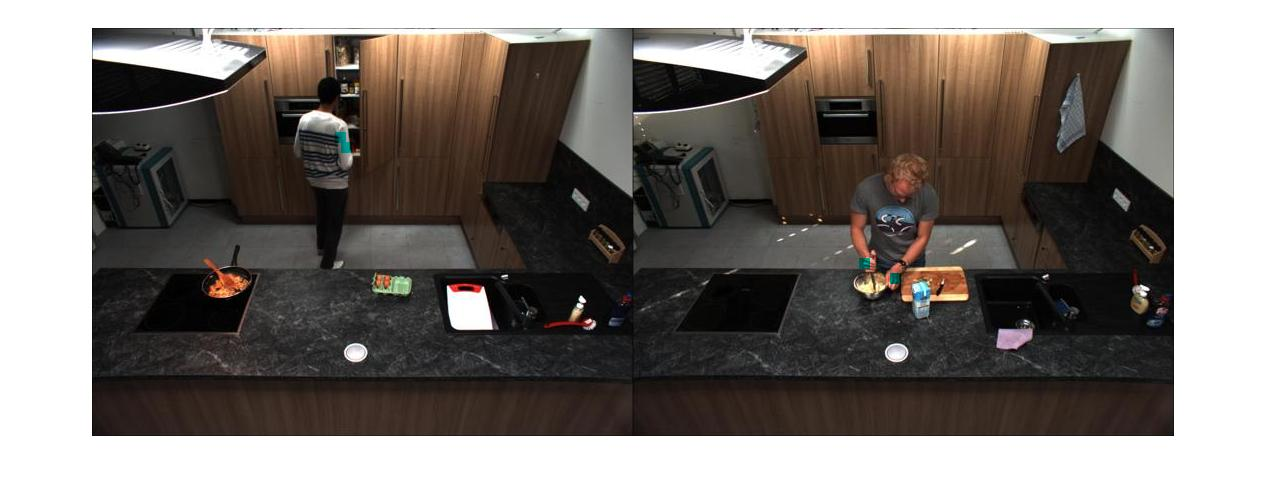
\includegraphics[scale=0.35]{{Images/AppHands}.jpg}}
  \caption{Παραδείγματα επισημειώσεων πόζας. Με μπλε απεικονίζονται τα σημεία που χαρακτηρίζονται ως χέρια μέσω των επισημειώσεων πόζας. Δείχνουμε τις περιοχες ως τετράγωνα $10 \times 10$ γύρω από τα σημεία επισημείωσης για να είναι εμφανείς οπτικά στον αναγνώστη. Βλέπουμε ότι ενώ στη δεξιά εικόνα οι επισημειώσεις ταυτίζονται με τη θέση των χεριών, τα οποία είναι εμφανή οπτικά, στην εικόνα αριστερά οι επισημειώσεις δείχνουν τη θέση που βρίσκεται το χέρι πίσω από το σώμα του ανθρώπου. Είναι φανερό ότι εικόνες σαν την αριστερή δεν μπορούν να χρησιμεύσουν σαν θετικά δείγματα για έναν ανιχνευτή χεριών και έτσι αποκλείονται από τα θετικά δεδομένα εκπαίδευσης και χρησιμοποιούντι μόνο για την εξαγωγή αρνητικών παραδειγμάτων.}
  \label{fig:AppHands}
\end{figure}



	% Appendix Title

%%\include{Appendices/AppendixB} % Appendix Title

%\input{Appendices/AppendixC} % Appendix Title
%\addtocontents{toc}{\vspace{2em}}  % Add a gap in the Contents, for aesthetics
%\end{appendices}
\backmatter

%% ----------------------------------------------------------------
\label{Bibliography}
\lhead{\emph{Βιβλιογραφία}}  % Change the left side page header to "Bibliography"
%\bibliographystyle{unsrtnat}  % Use the "unsrtnat" BibTeX style for formatting the Bibliography
\printbibliography
%\include{glossary}

\backmatter
\printindex
\end{document}  % The End
%% ----------------------------------------------------------------
